\chapter{Вычислительные эксперименты}
Рассматривается задача численного решения уравнения переноса скалярной величины \( u(x, y, t) \) в двумерной области \(\Omega \subset \mathbb{R}^2\). При отсутствии источников и стоков правая часть уравнения равна нулю (\(f = 0\)), и задача записывается в виде:

\begin{equation}
	\frac{\partial u}{\partial t} + \vec{v}(x, y, t) \cdot \nabla u = 0,
	\label{eq:advection}
\end{equation}

где \( \vec{v}(x, y, t) = (v_x, v_y) \) — заданное векторное поле скоростей, \( \nabla u = \left( \frac{\partial u}{\partial x}, \frac{\partial u}{\partial y} \right) \) — градиент функции \( u \).

Граничные условия принимаются периодическими. Начальное распределение \( u(x, y, 0) \) задается одной из аналитических функций: гауссовой функцией, индикатором круга и т.д.

\section{Аналитическое решение}

В случае отсутствия источников (\(f = 0\)) и известного поля скоростей \(\vec{v}(x,y,t)\), уравнение \eqref{eq:advection} допускает аналитическое решение вдоль траекторий частиц, заданных уравнением:

\begin{equation}
	\frac{d\vec{x}}{dt} = \vec{v}(\vec{x}, t), \quad \vec{x}(0) = \vec{x}_0,
	\label{eq:characteristics}
\end{equation}

где \(\vec{x}_0\) — начальная координата частицы. Тогда значение скалярной величины \(u\) вдоль характеристики сохраняется:

\begin{equation}
	u(\vec{x}(t), t) = u_0(\vec{x}_0).
	\label{eq:solution_along_characteristics}
\end{equation}

Это решение реализуется в методе лагранжевых частиц.
\section{Программа для ЭВМ}
В качестве языка программирования для рассчётов и
визуализации был выбран Python с использованием библиотек numpy
(вычисления) и matplotlib (визуализация).
\section{Ввех по потоку (upwind)}
\subsection{Численная схема конечных разностей}

Пространственная область \(\Omega = [x_{\min}, x_{\max}] \times [y_{\min}, y_{\max}]\) дискретизуется равномерной сеткой с \(n \times n\) узлами. Шаги по пространству:

\[
dx = \frac{x_{\max} - x_{\min}}{n - 1}, \quad dy = \frac{y_{\max} - y_{\min}}{n - 1}.
\]

Для аппроксимации производных используются односторонние разности в зависимости от направления скорости (схема upwind):

\[
\frac{\partial u}{\partial x} \approx
\begin{cases}
	\frac{u_{i,j} - u_{i-1,j}}{dx}, & v_x \geq 0 \\
	\frac{u_{i+1,j} - u_{i,j}}{dx}, & v_x < 0
\end{cases}, \quad
\frac{\partial u}{\partial y} \approx
\begin{cases}
	\frac{u_{i,j} - u_{i,j-1}}{dy}, & v_y \geq 0 \\
	\frac{u_{i,j+1} - u_{i,j}}{dy}, & v_y < 0
\end{cases}
\]

Временное интегрирование производится явным способом (метод Эйлера):

\[
u_{i,j}^{n+1} = u_{i,j}^{n} - \Delta t \left( v_x \frac{\partial u}{\partial x} + v_y \frac{\partial u}{\partial y} \right).
\]

Стабильность обеспечивается условием Куранта–Фридрихса–Леви (CFL):

\begin{equation}
	\max \left( \frac{|v_x| \Delta t}{dx}, \frac{|v_y| \Delta t}{dy} \right) \leq 1.
	\label{eq:cfl_condition}
\end{equation}

\subsection{Описание экспериментов}

В ходе экспериментов используются различные поля скоростей:
\begin{itemize}
	\item \textbf{Вихревое течение (vortex)}:
	\begin{equation}
			v_x = -\alpha (y - y_c), \quad v_y = \alpha (x - x_c),
			\label{eq:vortex}
	\end{equation}
	где \(\alpha = 0.1\), \(x_c = y_c = 5\).
	
	\item \textbf{Сдвиговое течение (shear)}:
	\begin{equation}
			v_x = 0.7(1 + \sin(y + 0.5)), \quad v_y = 0.15 \cos(x + 0.3).
			\label{eq:shear}
	\end{equation}

	
	\item \textbf{Дивергентное поле (divergance)}:
	\begin{equation}
			v_x = -\pi \sin\left( \frac{2\pi x}{10} \right) \cos\left( \frac{\pi y}{10} \right), \quad
		v_y = 2\pi \sin\left( \frac{\pi y}{10} \right) \cos\left( \frac{2\pi x}{10} \right).
		\label{eq:div}
	\end{equation}

\end{itemize}

Начальные условия представлены в виде кругов или гауссовых распределений.

\subsection{Реализация алгоритма на Python}

Программа реализована на языке Python с использованием библиотек \texttt{numpy} и \texttt{matplotlib}. Структура кода включает:
\begin{itemize}
	\item \texttt{FluidSimulation} — класс с основной логикой метода конечных разностей;
	\item \texttt{VelocityField} — статические методы для задания различных полей скоростей;
	\item \texttt{InitialCondition} — начальные условия;
	\item \texttt{Experiment}, \texttt{ExperimentManager} — система организации и запуска экспериментов;
	\item визуализация полей скоростей и решений.
\end{itemize}

Пример вставки кода:
\begin{lstlisting}[language=Python, caption={Основной цикл аппроксимации переноса}, label={lst:fd_loop}]
	for i in range(1, n - 1):
	for j in range(1, n - 1):
	if vx[j, i] >= 0:
	du_dx = (u[j, i] - u[j, i - 1]) / dx
	else:
	du_dx = (u[j, i + 1] - u[j, i]) / dx
	
	if vy[j, i] >= 0:
	du_dy = (u[j, i] - u[j - 1, i]) / dy
	else:
	du_dy = (u[j + 1, i] - u[j, i]) / dy
	
	u_new[j, i] = u[j, i] - dt * (vx[j, i] * du_dx + vy[j, i] * du_dy)
\end{lstlisting}


Все течения зададим стационарными (не зависящими от $t$)
\subsection{Визуализация результатов}

Результаты каждого эксперимента сохраняются в виде изображений, иллюстрирующих:
\begin{itemize}
	\item исходное распределение скалярной величины \(u(x,y,0)\);
	\item поле скоростей (стримплот);
	\item распределение \(u(x,y,t)\) на каждом шаге.
\end{itemize}

\subsection{Вихревое течение}
\begin{figure}[h]
	\centering
	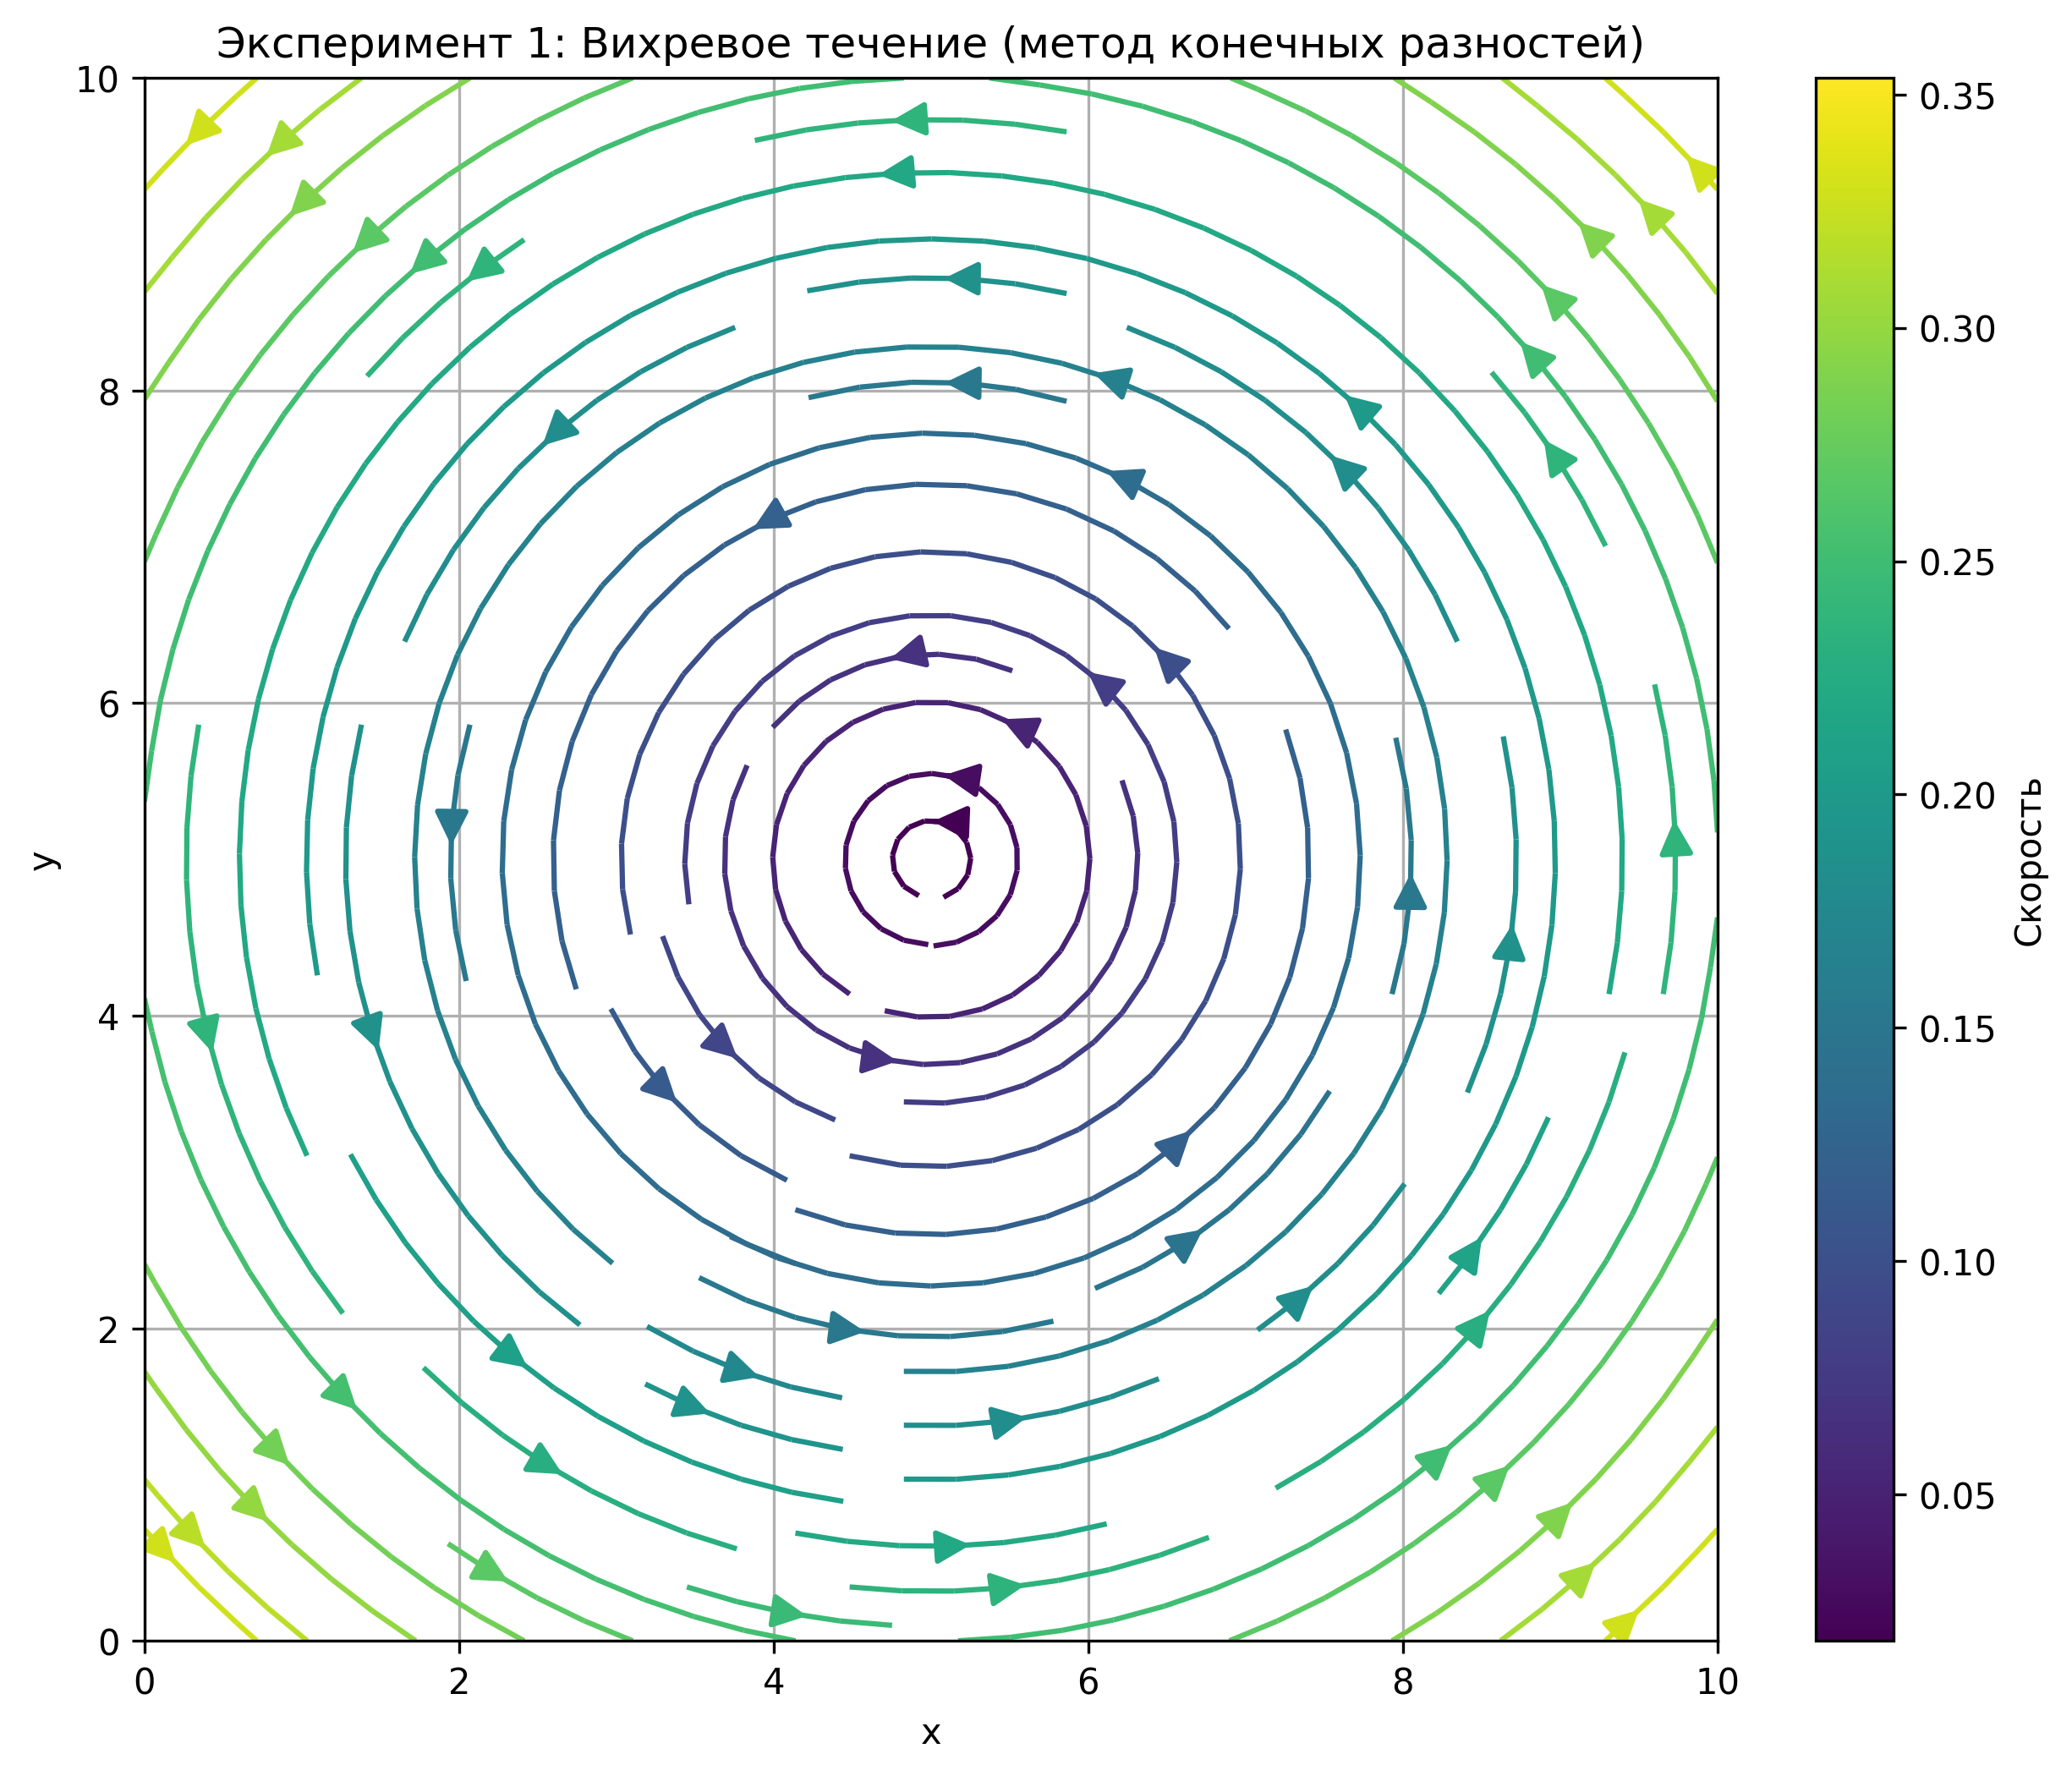
\includegraphics[width=0.7\textwidth]{imgs/эксперимент_1:_вихревое_течение_fd_velocity_field.png}
	\caption{Поле скоростей для вихревого течения}
	\label{fig:vortex_velocity}
\end{figure}
Поле на рис. \ref{fig:vortex_velocity} задаётся уравнением вихря (\ref{eq:vortex}):

В качестве начального распределения, используется круг с центром в точке (2.5 , 5) и радиусом 3 (\ref{fig:vortex_begin}).
\begin{figure}
	\centering
	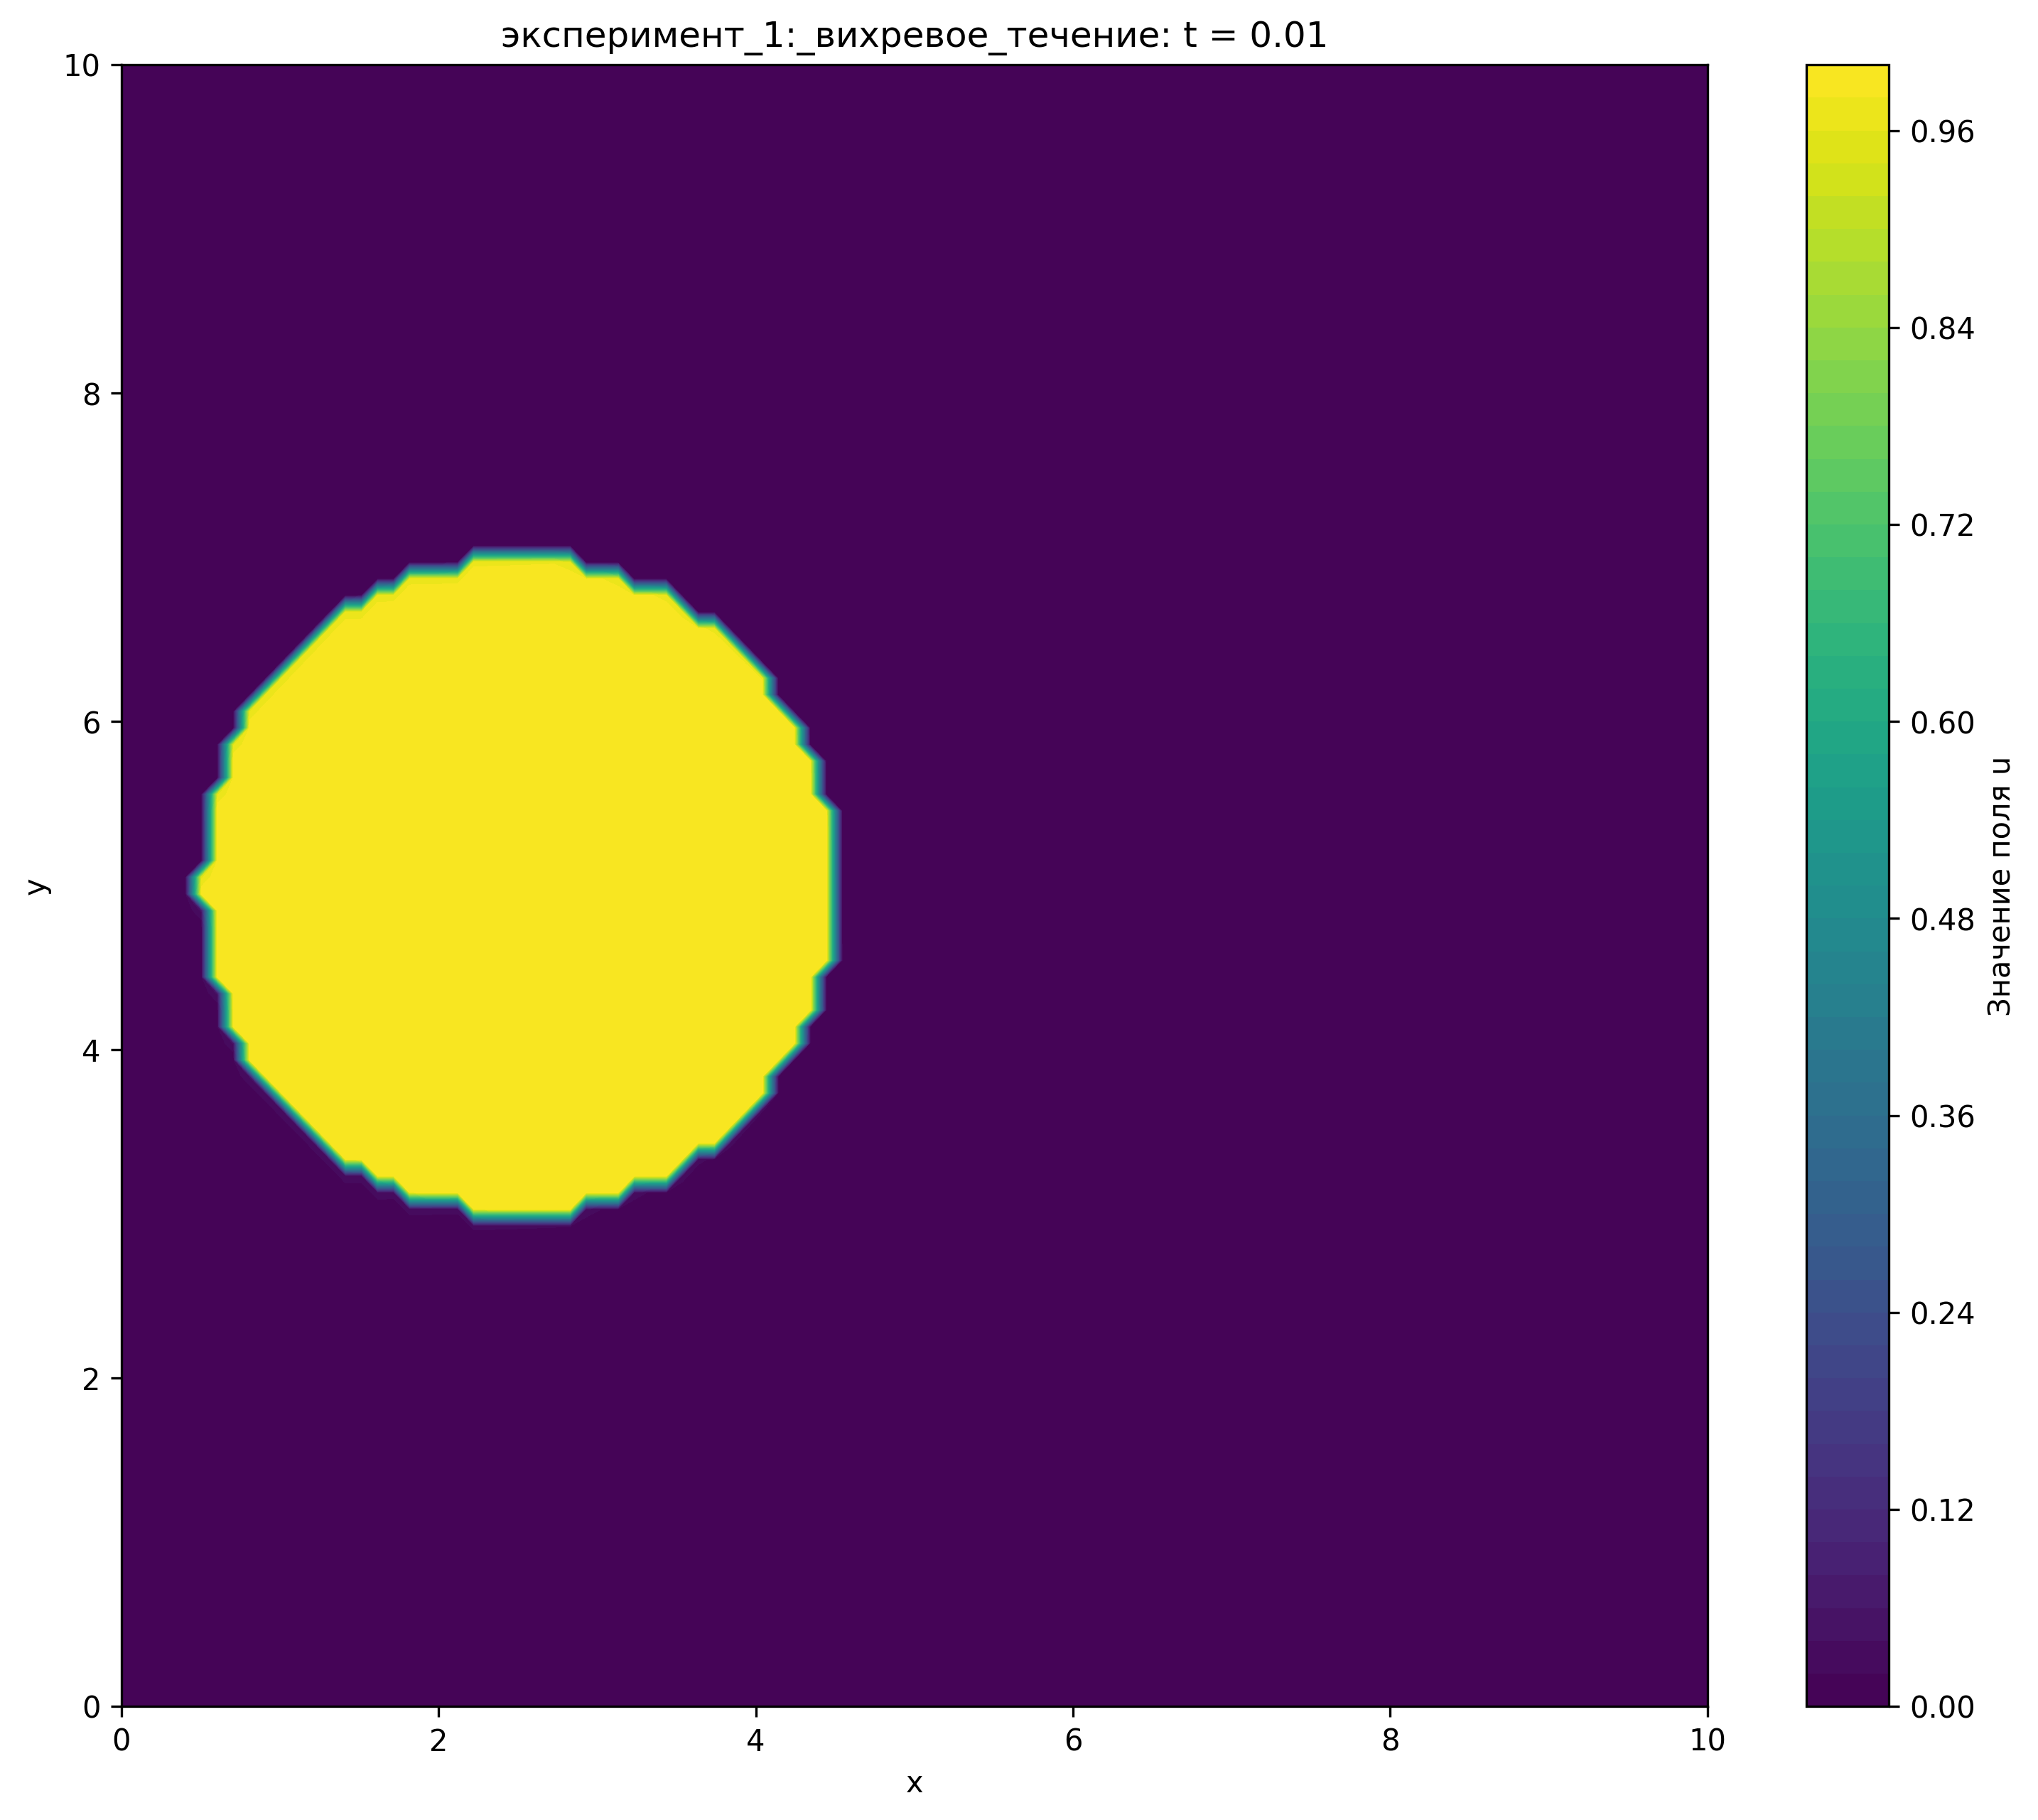
\includegraphics[width=0.7\textwidth]{imgs/эксперимент_1:_вихревое_течение_t0.01.png}
	\caption{Скалярное поле \(u(x,y,T)\) в начальный момент времени (0) (вихревое течение)}
	\label{fig:vortex_begin}
\end{figure}
Изображения промежуточных ходов представлены в приложении (ВСТАВИТЬ ССЫЛКУ НА ПРИЛОЖЕНИЕ)
Финальное распределения  представлено на рис. \ref{fig:vortex_final}:
\begin{figure}
	\centering
	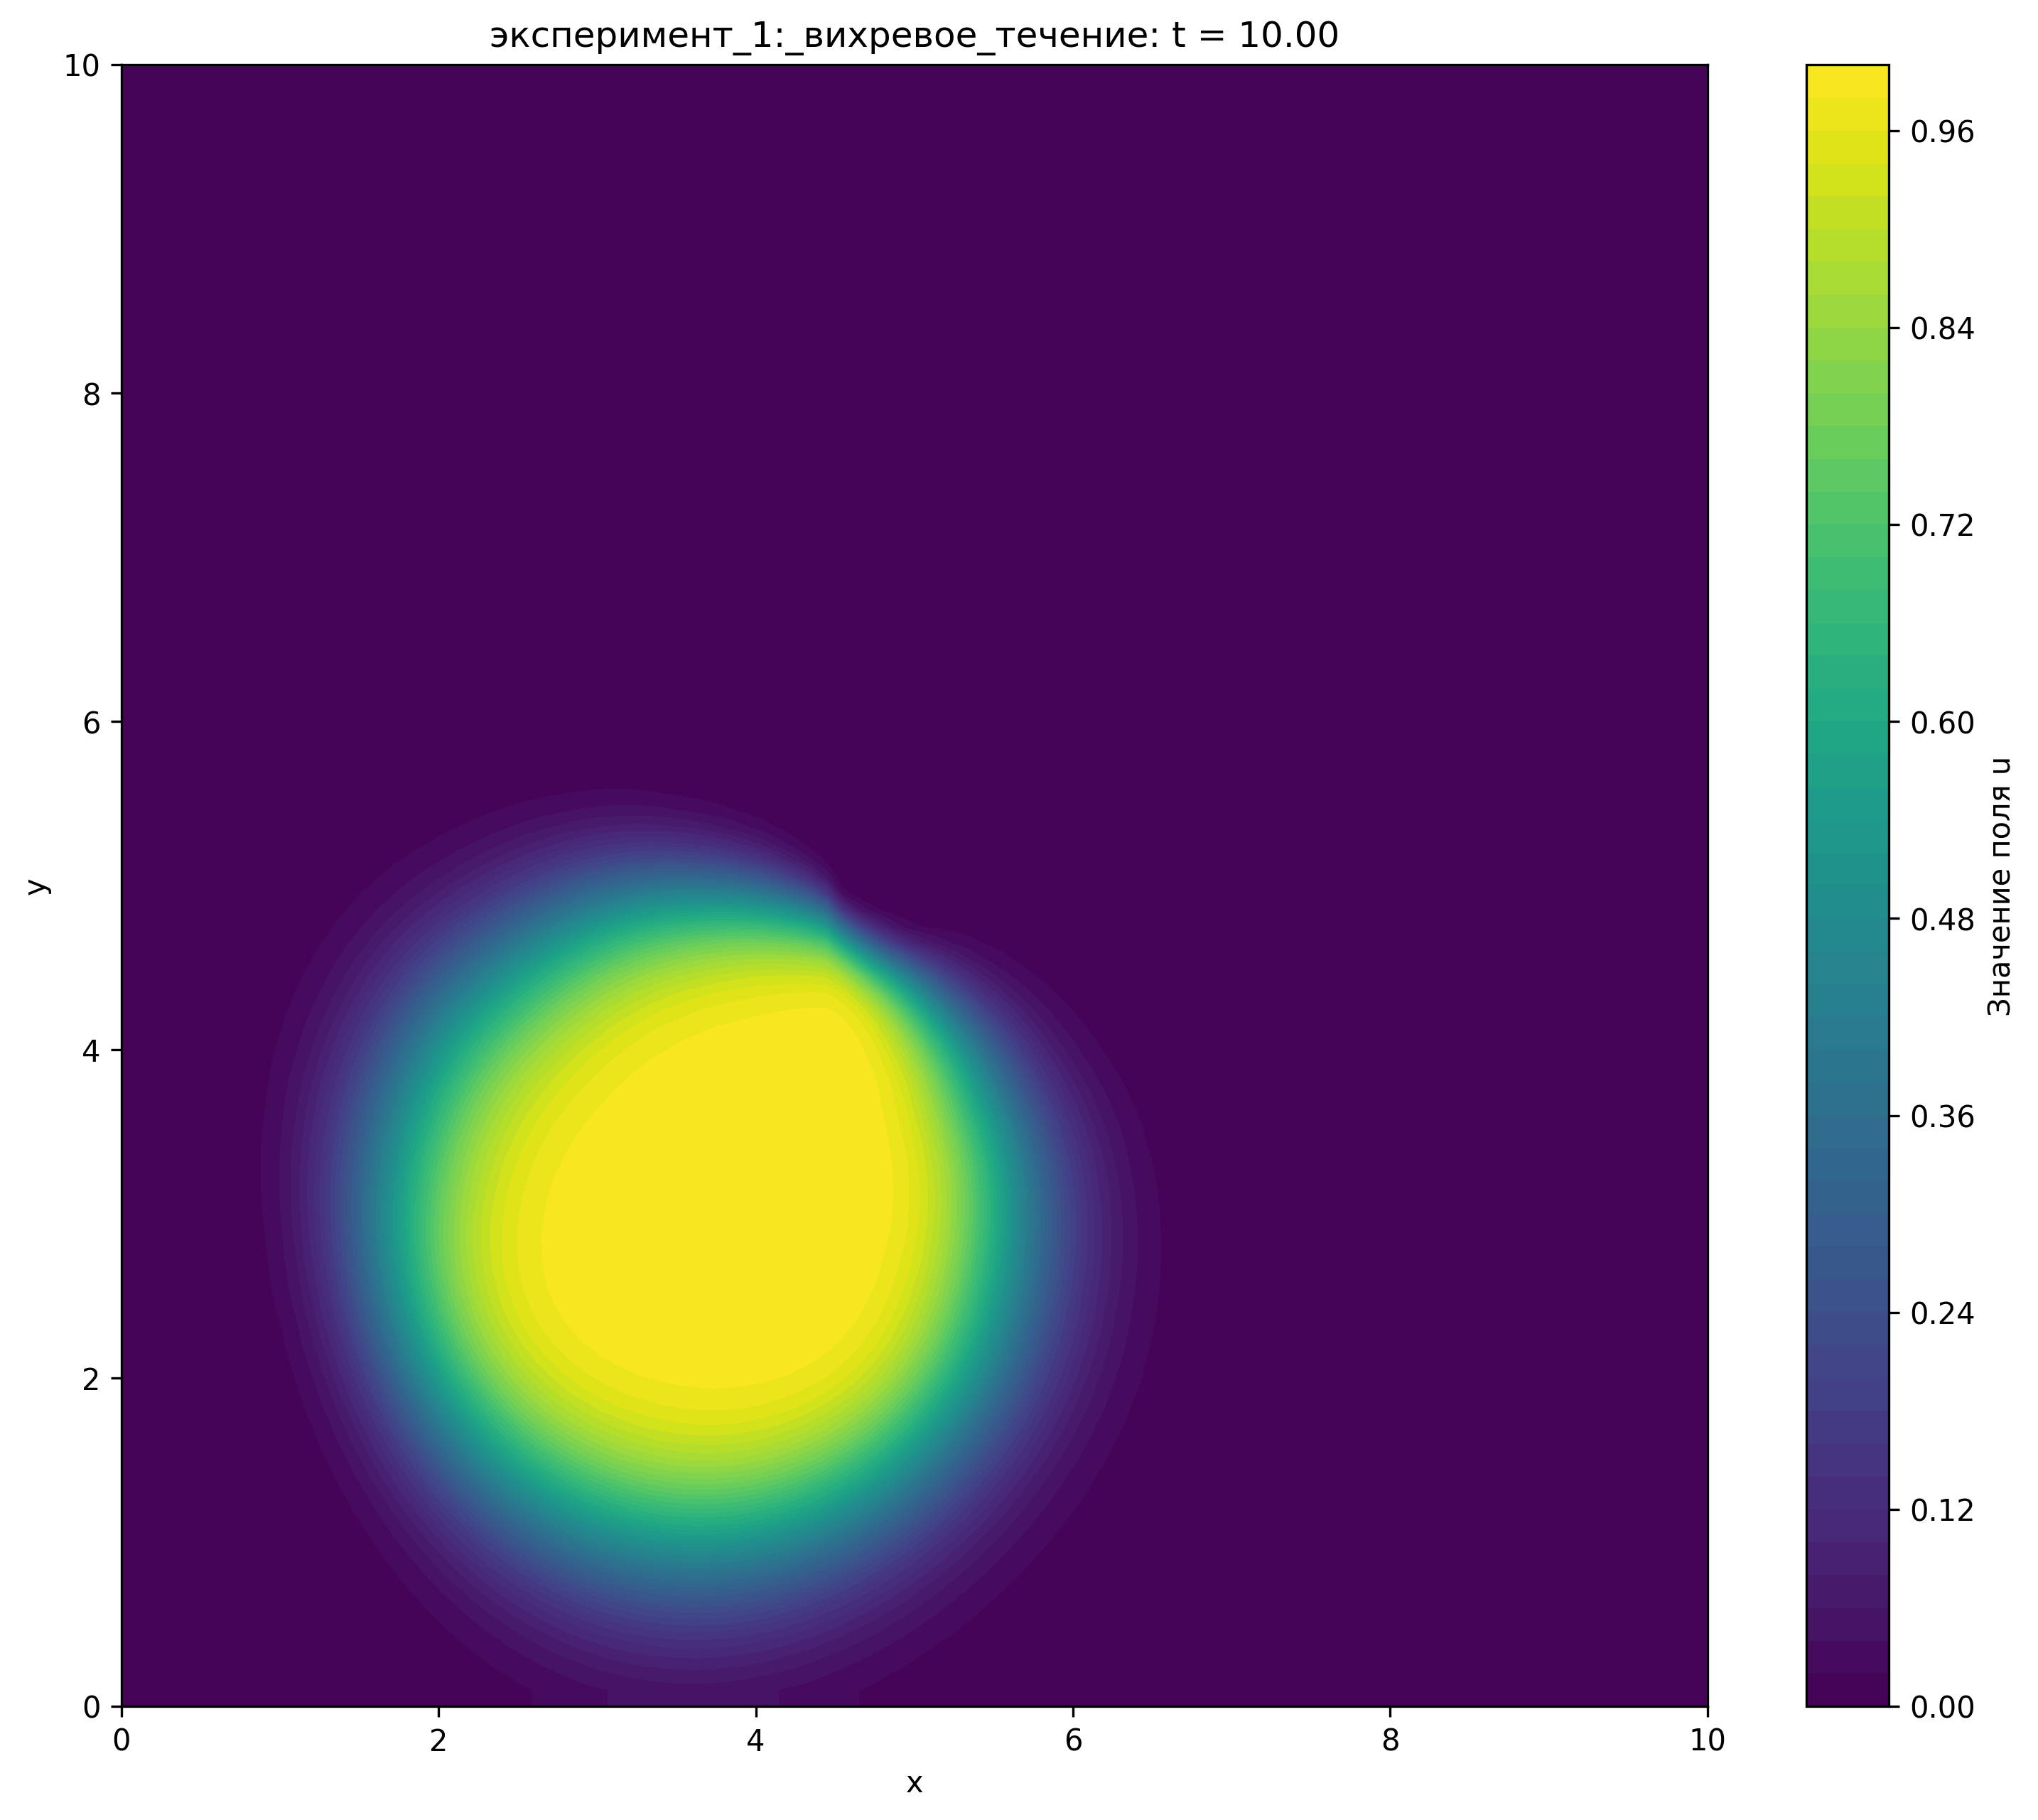
\includegraphics[width=0.7\textwidth]{imgs/эксперимент_1:_вихревое_течение_t10.00.png}
	\caption{Скалярное поле \(u(x,y,T)\) в финальный момент времени (10) (вихревое течение)}
	\label{fig:vortex_final}
\end{figure}
\newpage
\subsection{Cдвиговое течение}
Поле на рис. \ref{fig:shear_velocity} задаётся уравнением поля (\ref{eq:shear})
\begin{figure}
	\centering
	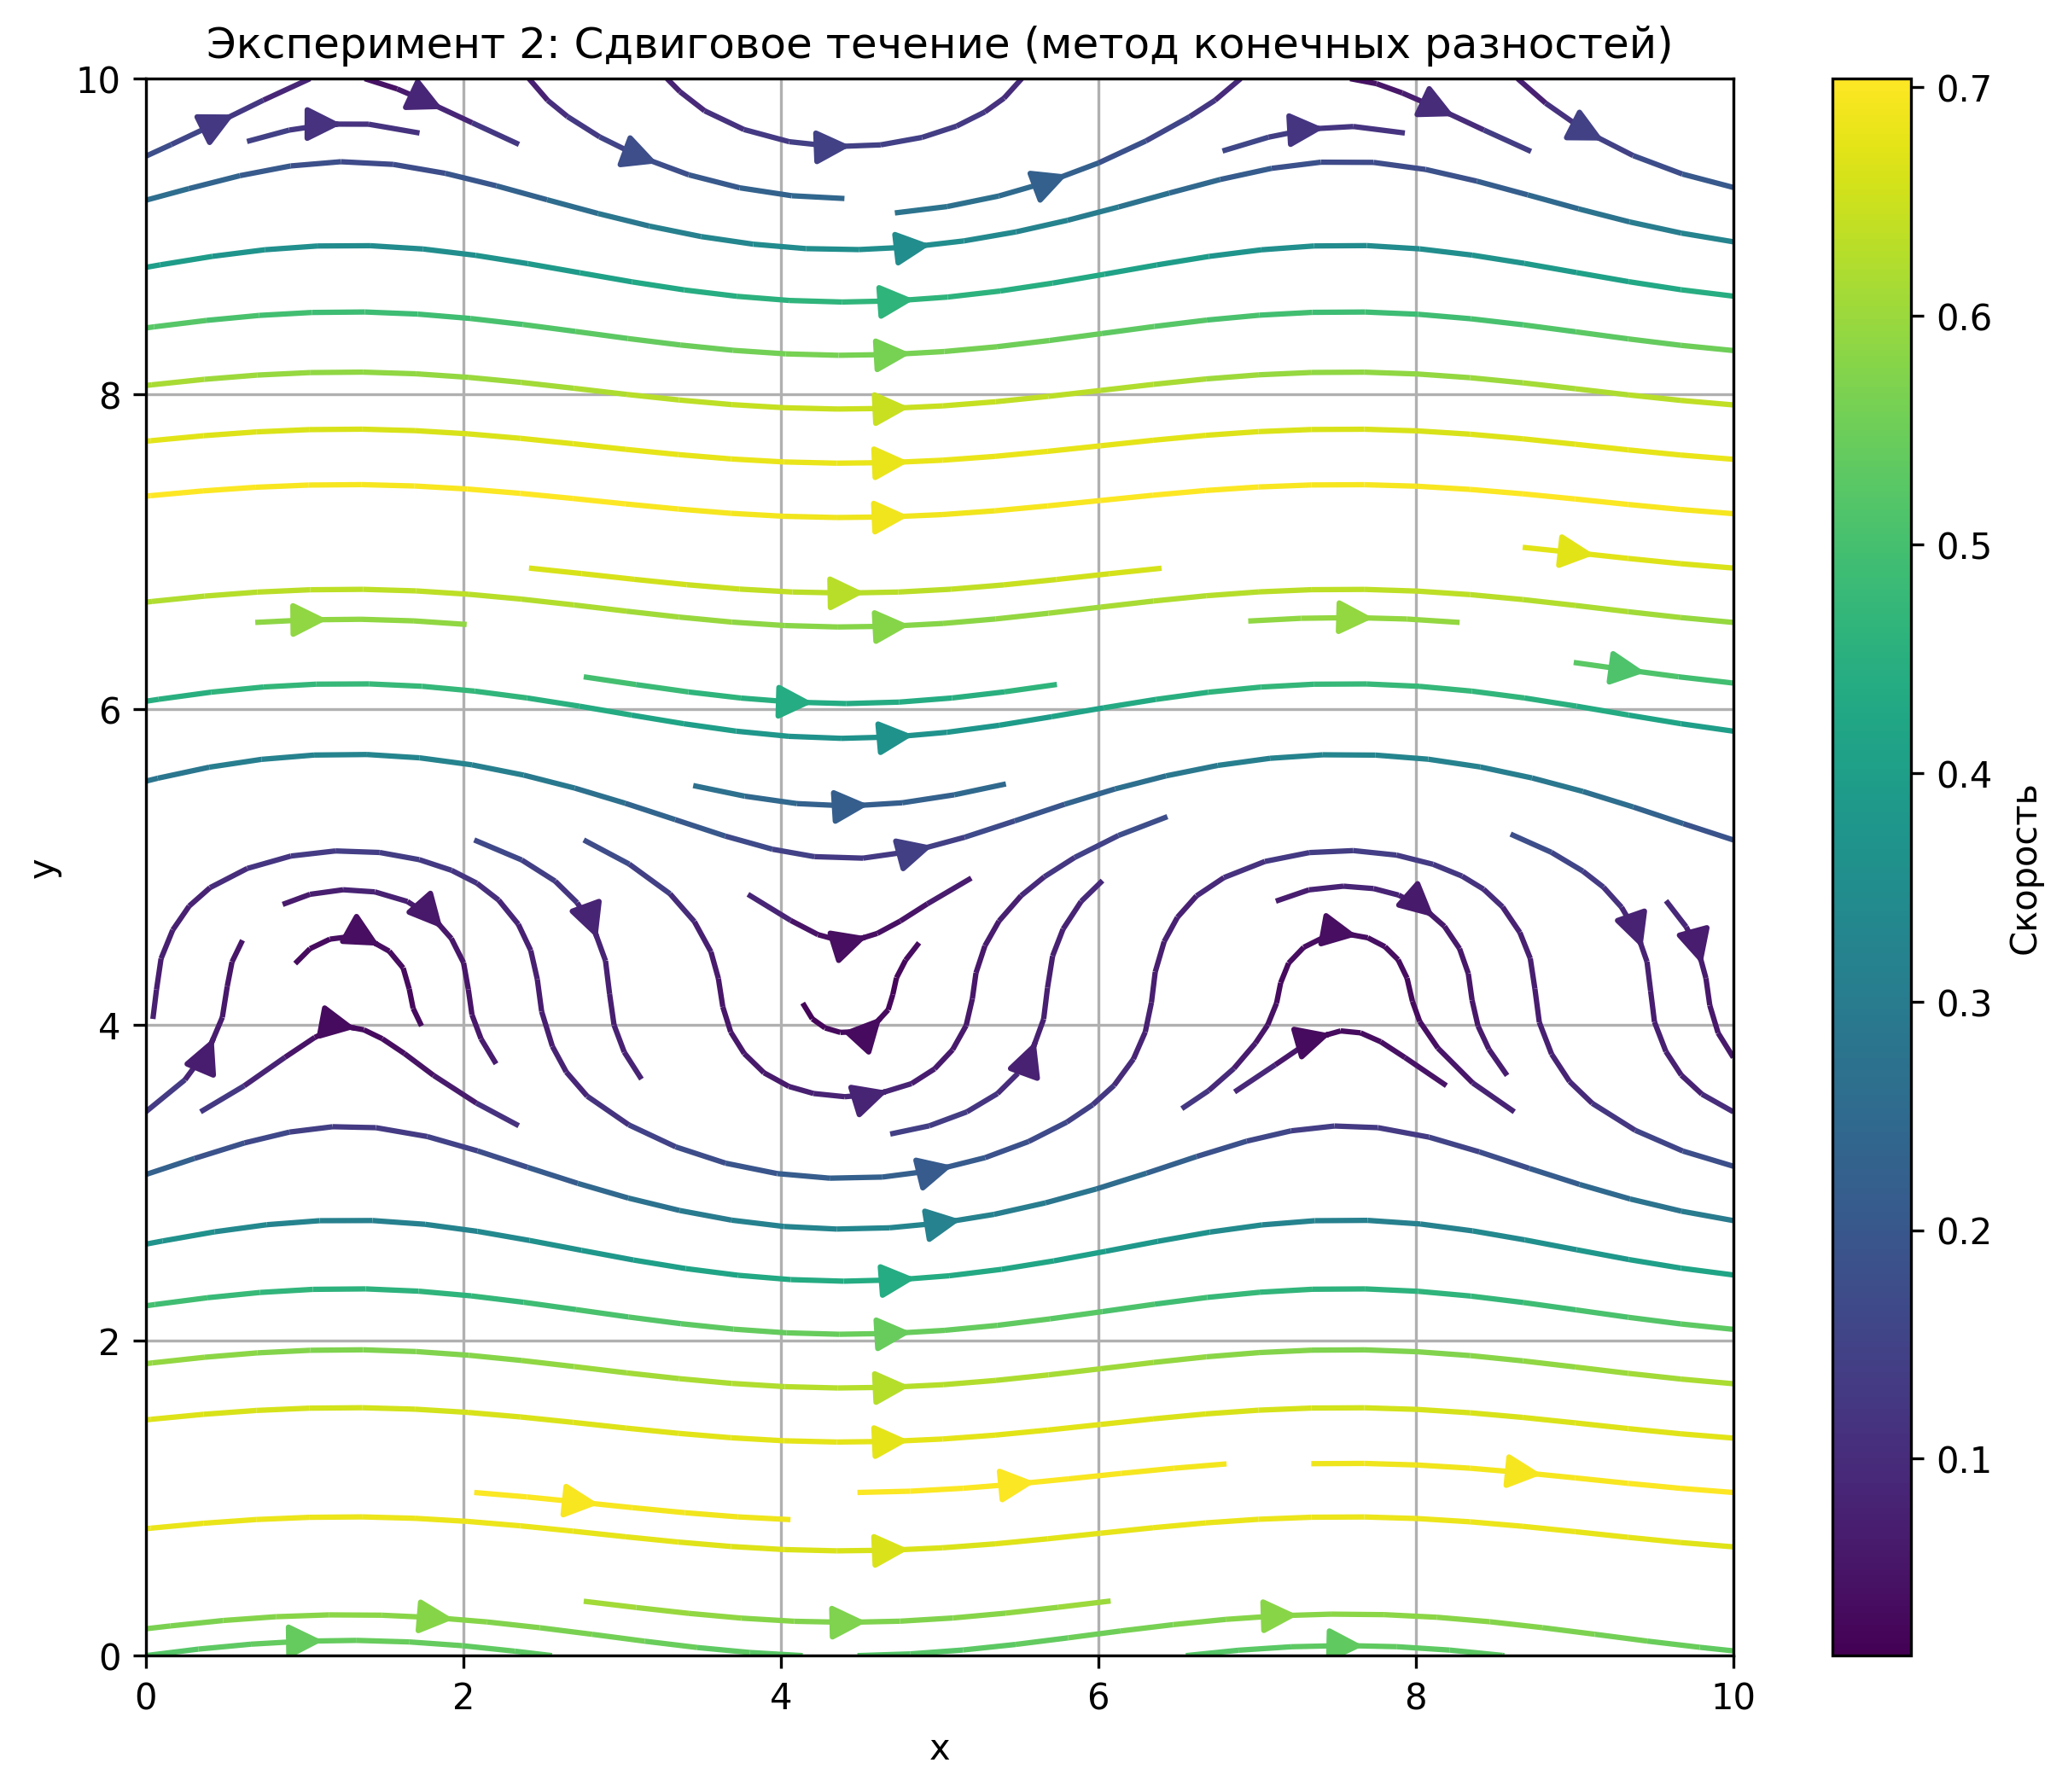
\includegraphics[width=0.7\textwidth]{imgs/эксперимент_2:_сдвиговое_течение_fd_velocity_field.png}
	\caption{Поле скоростей для сдвигового течения}
	\label{fig:shear_velocity}
\end{figure}

В качетве начального распределения, используется круг с центром в точке (5 , 5) и радиусом 2 ( рис. \ref{fig:shear_begin}).
\begin{figure}
	\centering
	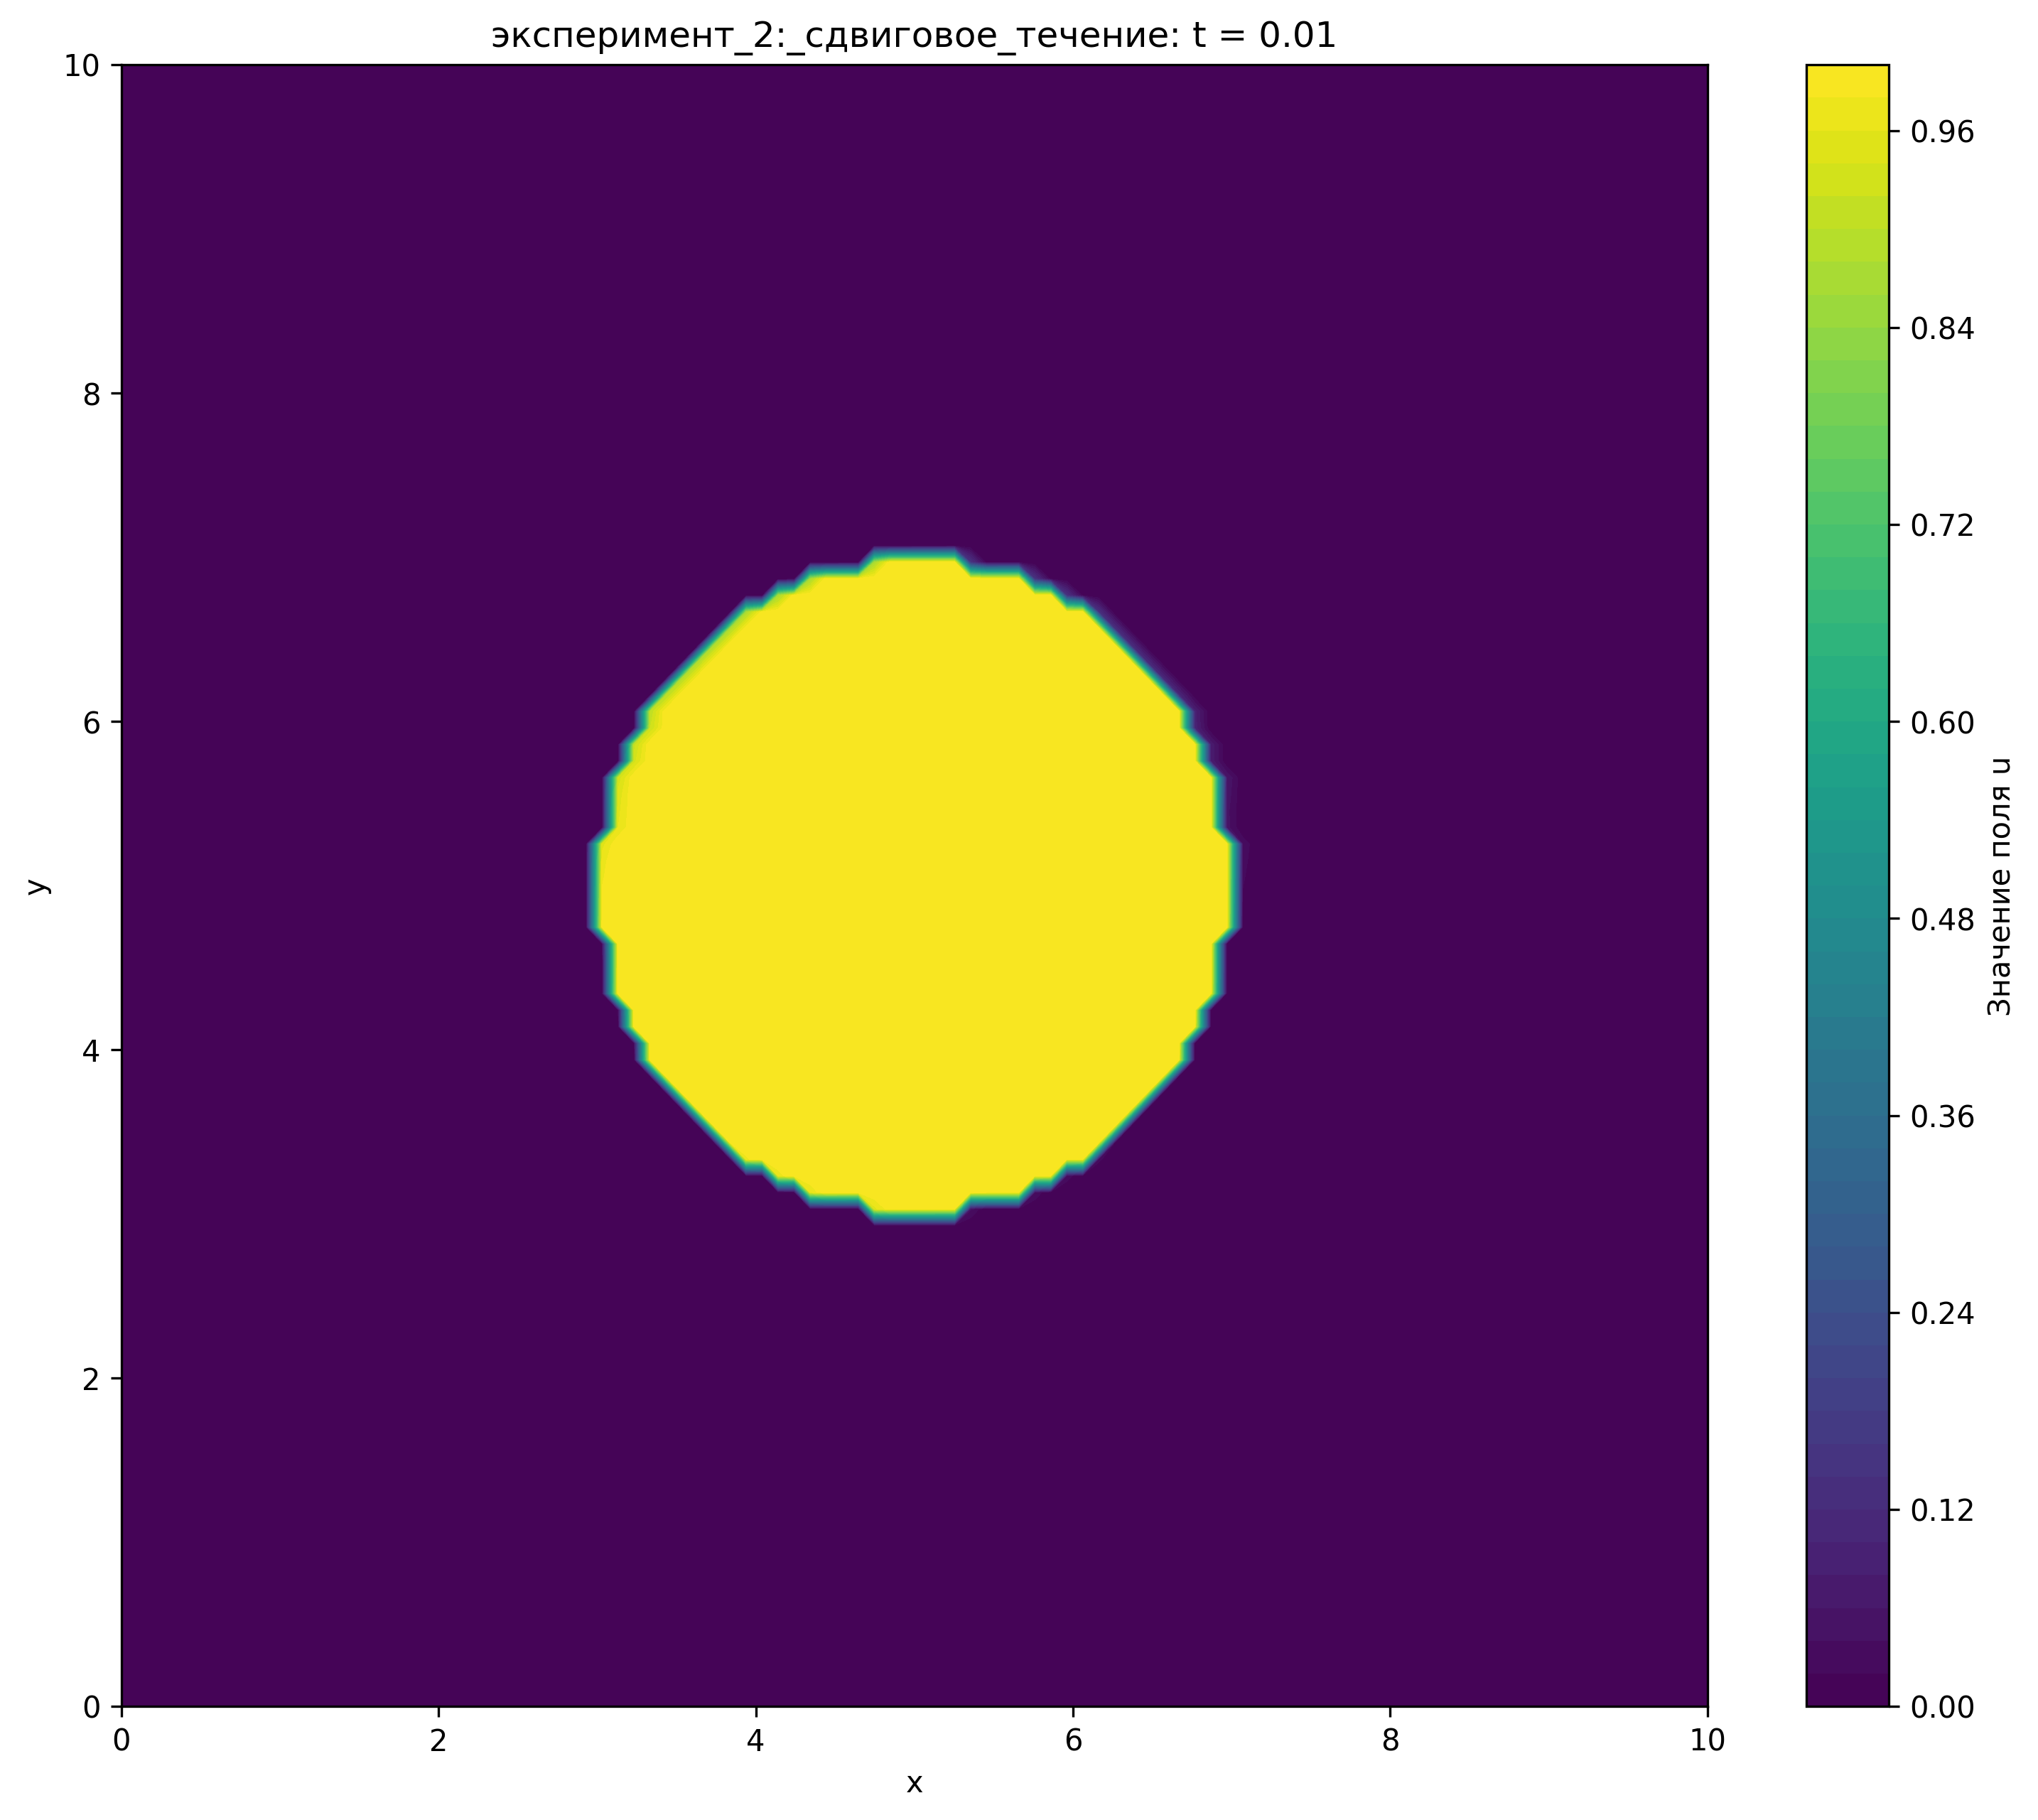
\includegraphics[width=0.7\textwidth]{imgs/эксперимент_2:_сдвиговое_течение_t0.01.png}
	\caption{Скалярное поле \(u(x,y,T)\) в начальный момент времени (0) (вихревое течение)}
	\label{fig:shear_begin}
\end{figure}

Изображения промежуточных ходов представлены в приложении (ВСТАВИТЬ ССЫЛКУ НА ПРИЛОЖЕНИЕ)

Финальное распределения представлено на рис. \ref{fig:shear_final}.

\begin{figure}
	\centering
	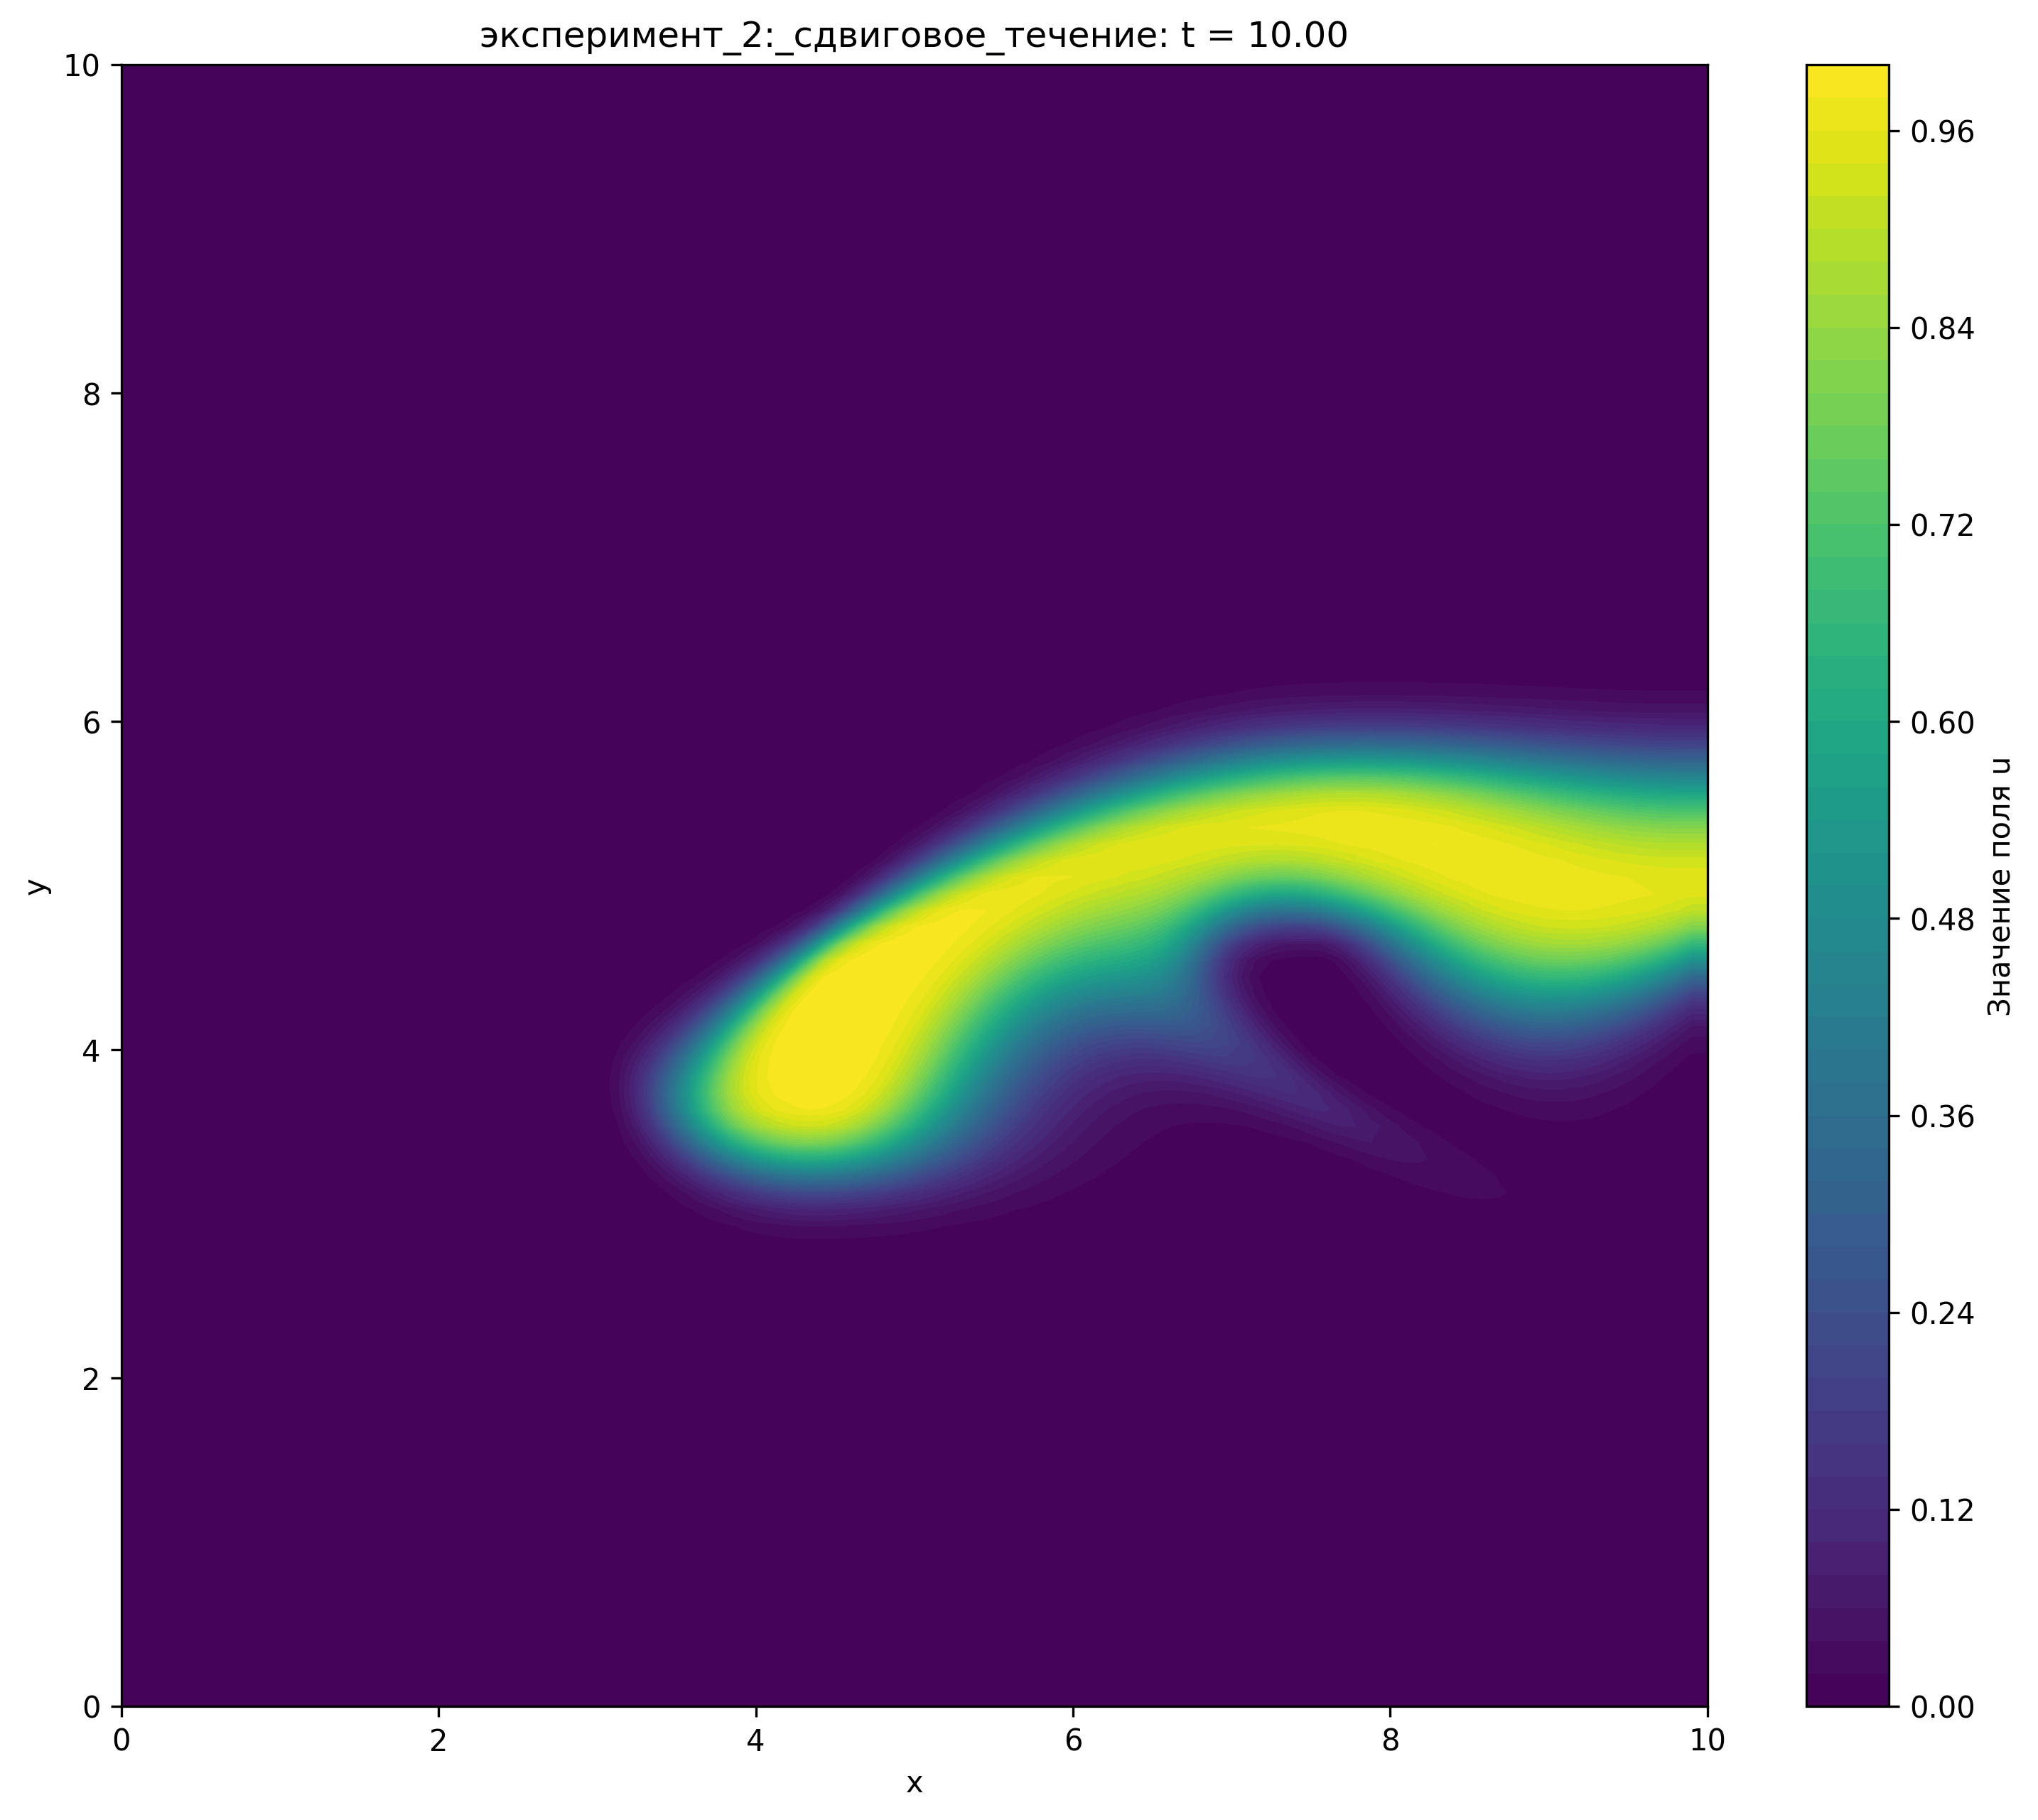
\includegraphics[width=0.7\textwidth]{imgs/эксперимент_2:_сдвиговое_течение_t10.00.png}
	\caption{Скалярное поле \(u(x,y,T)\) в финальный момент времени (10) (вихревое течение)}
	\label{fig:shear_final}
\end{figure}
\newpage
\subsection{Дивергентное течение}
Поле на рис. \ref{fig:div_velocity} задаётся уравнением поля (\ref{eq:div}):
\begin{figure}[h]
	\centering
	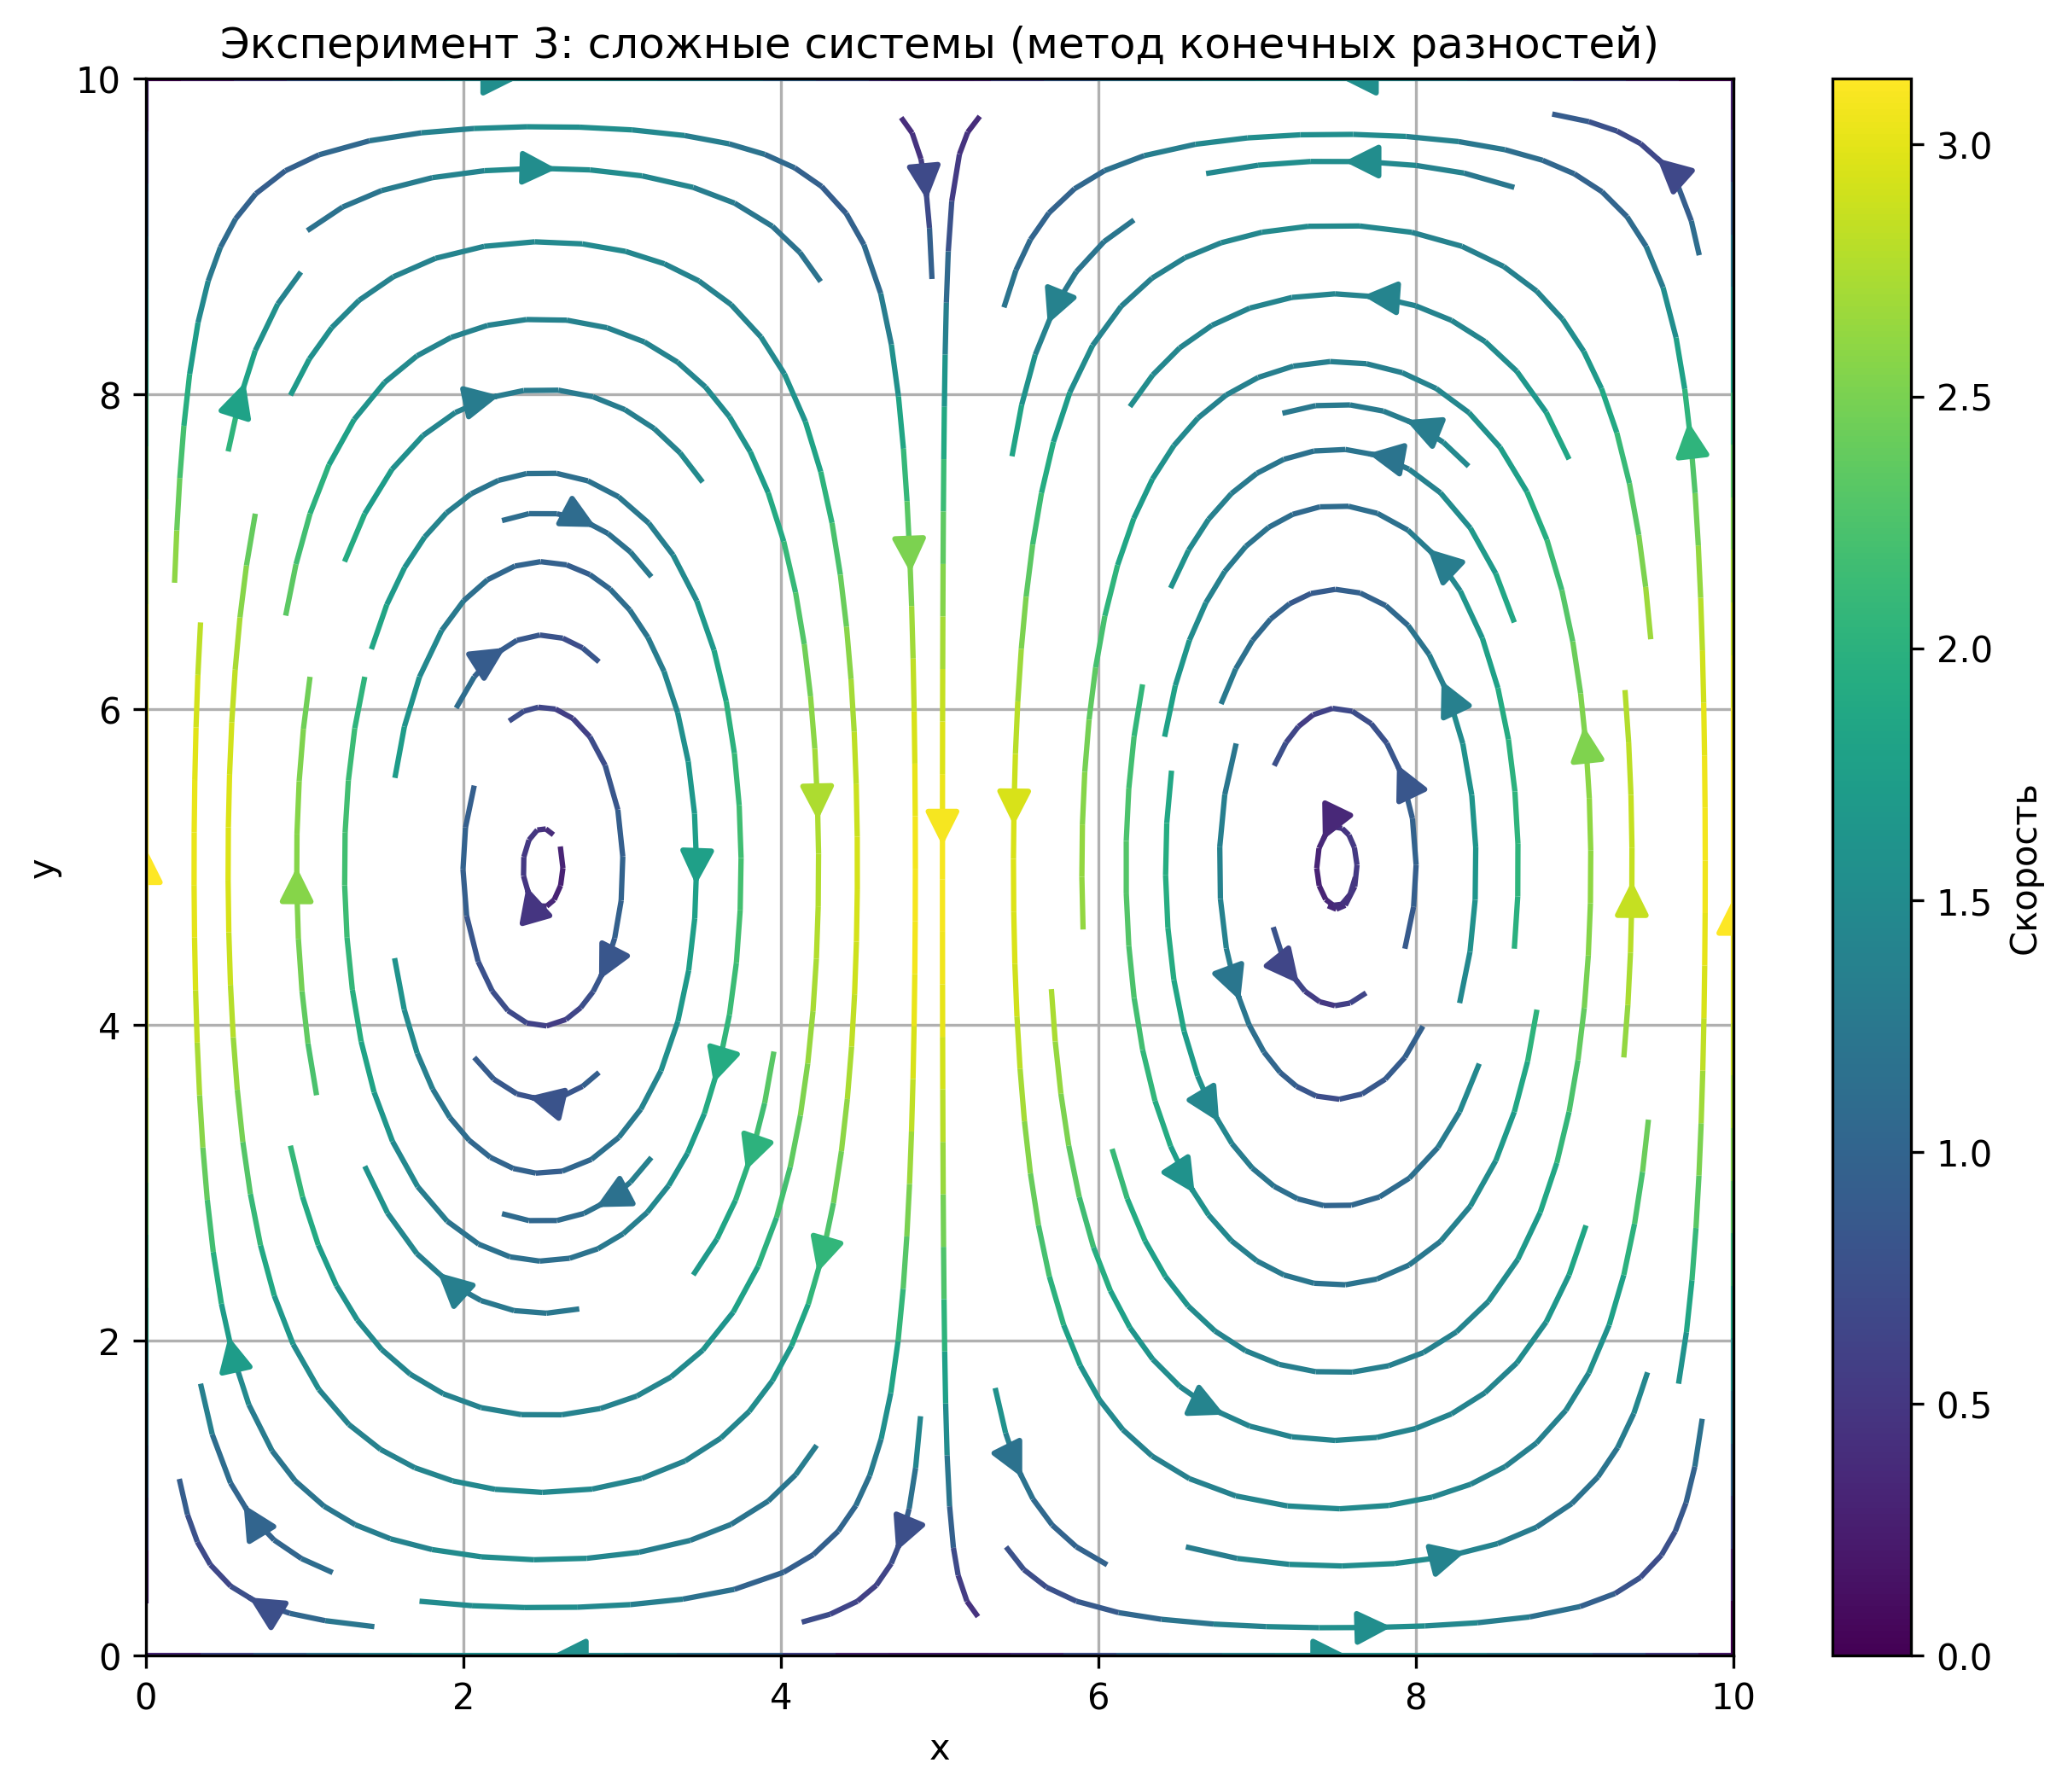
\includegraphics[width=0.7\textwidth]{imgs/эксперимент_3:_сложные_системы_fd_velocity_field.png}
	\caption{Поле скоростей для Дивергентного течения}
	\label{fig:div_velocity}
\end{figure}
В качетве начального распределения, используется круг с центром в точке (5 , 5) и радиусом 2 ( рис. \ref{fig:div_begin}).
\begin{figure}
	\centering
	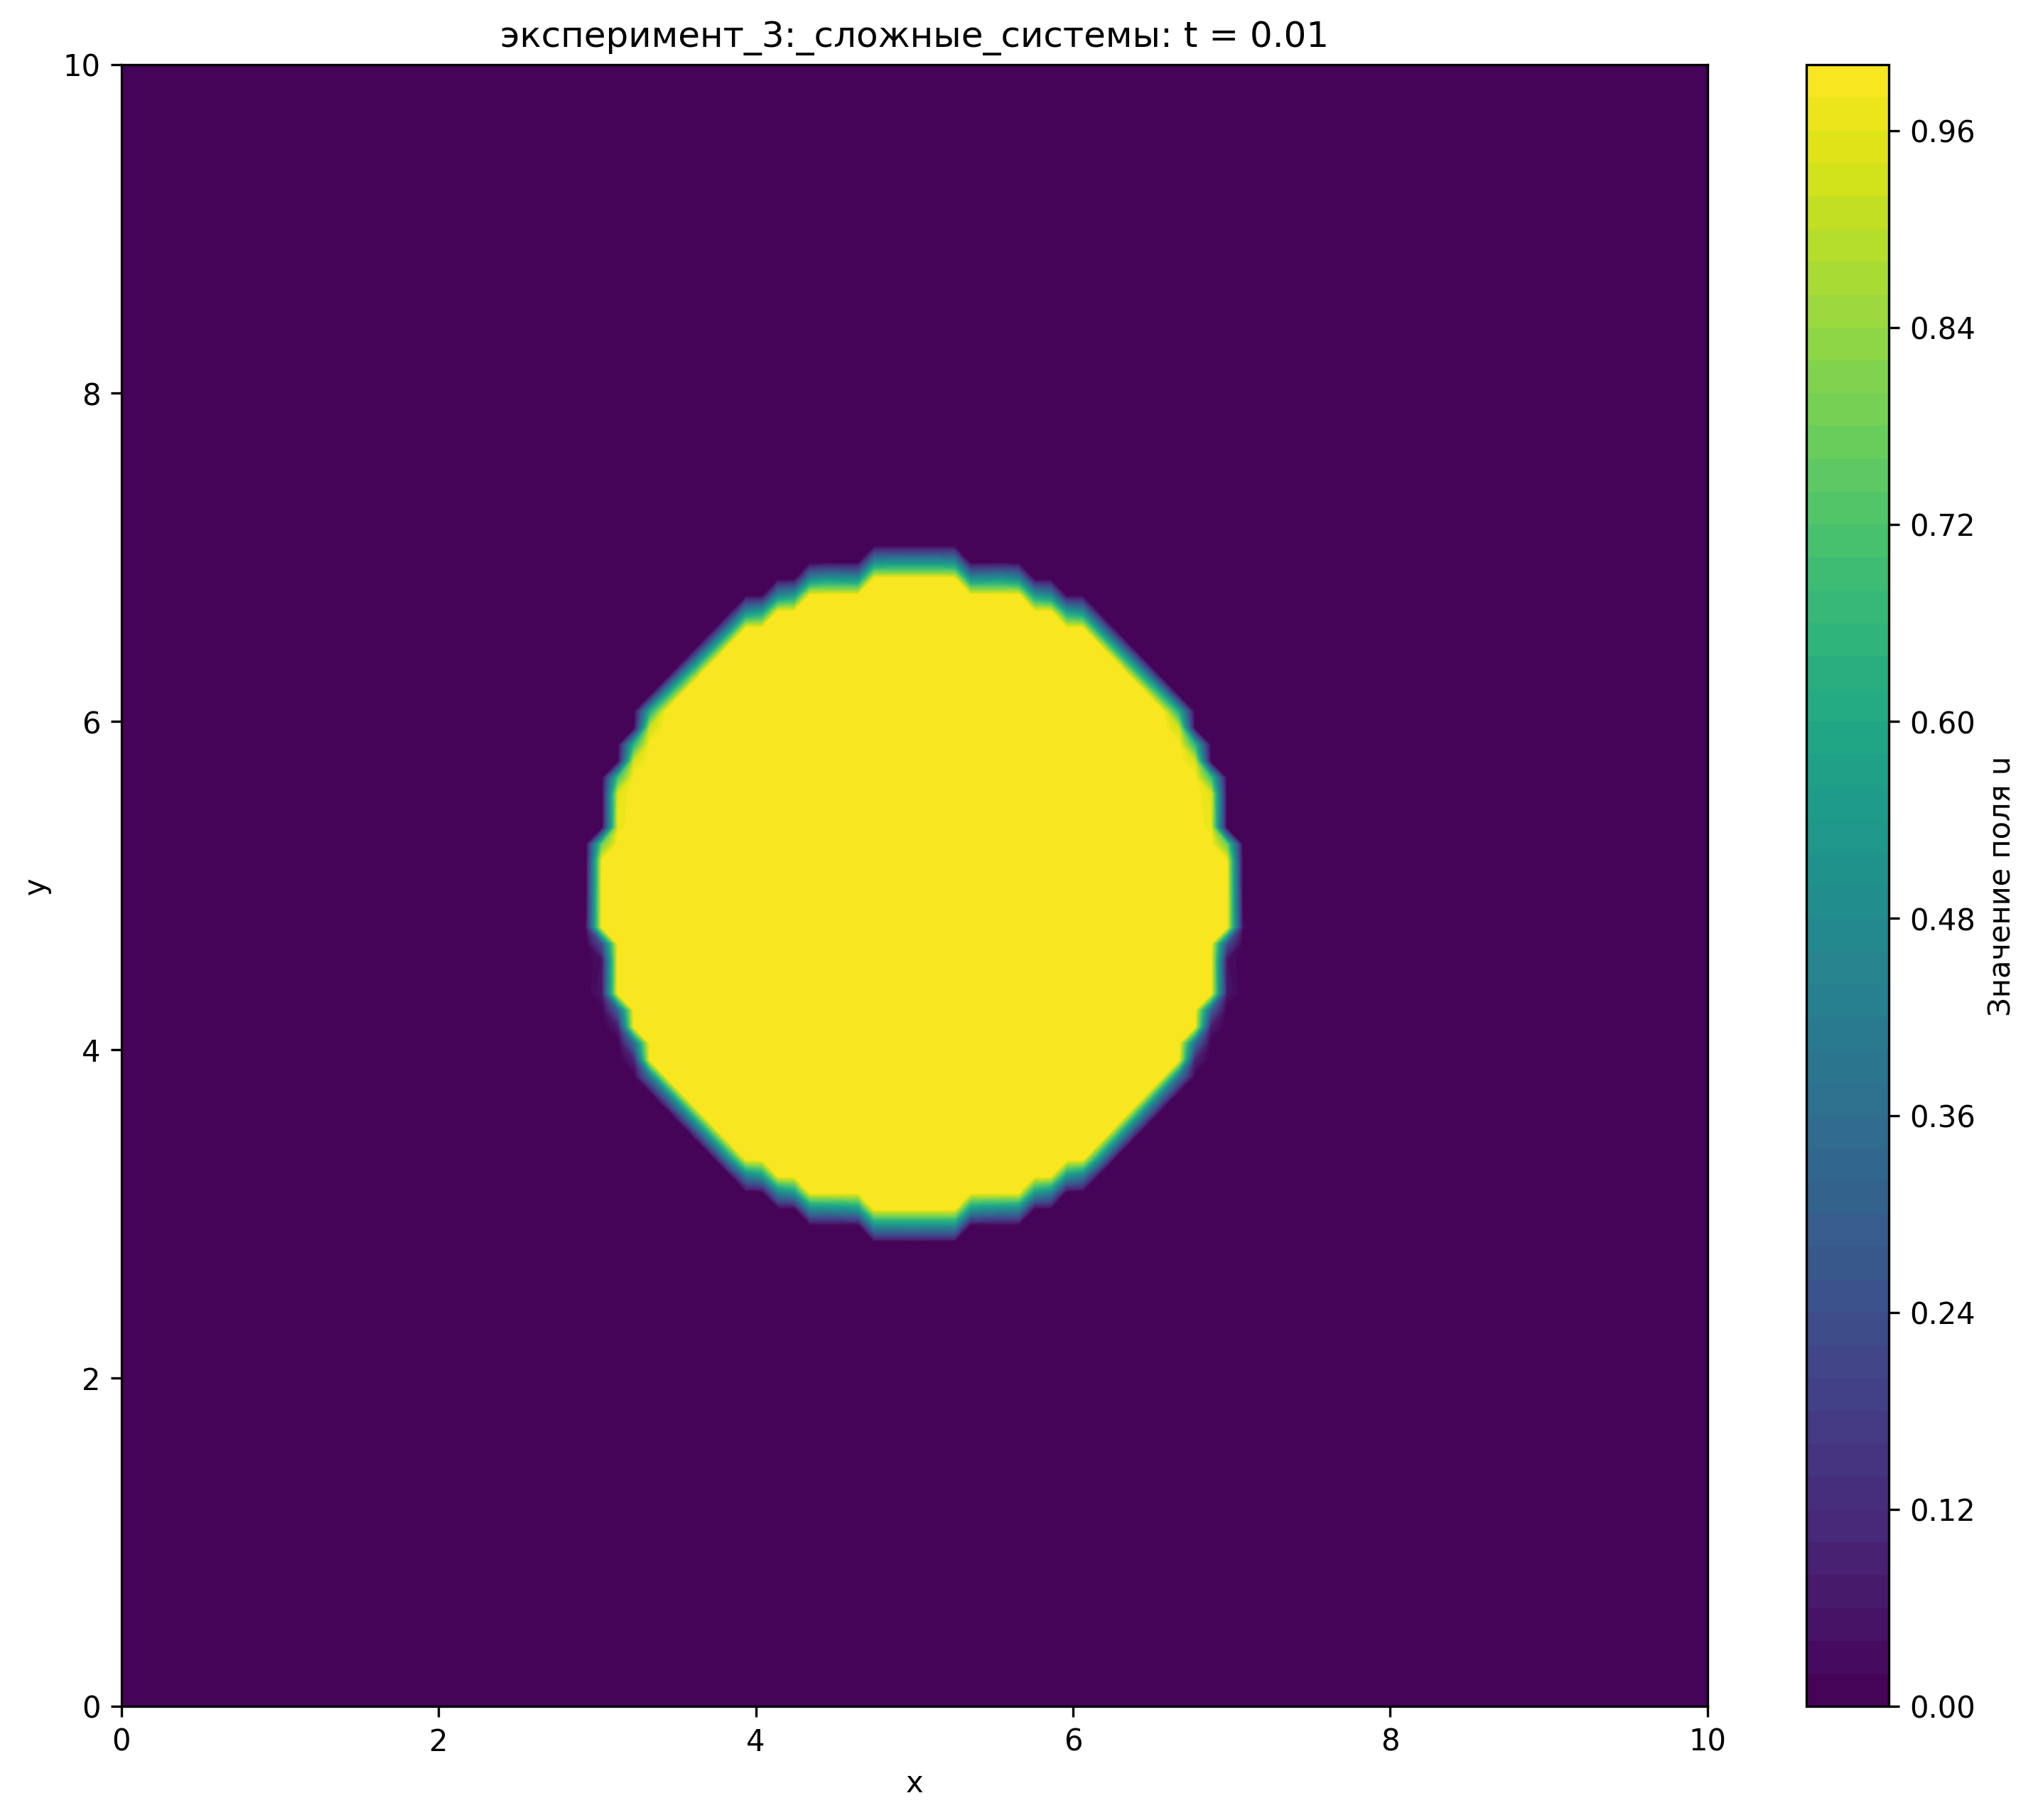
\includegraphics[width=0.7\textwidth]{imgs/эксперимент_3:_сложные_системы_t0.01.png}
	\caption{Скалярное поле \(u(x,y,T)\) в начальный момент времени (0) (вихревое течение)}
	\label{fig:div_begin}
\end{figure}
Изображения промежуточных ходов представлены в приложении (ВСТАВИТЬ ССЫЛКУ НА ПРИЛОЖЕНИЕ)
Финального распределение представлено на рис. \ref{fig:div_final}.
\begin{figure}
	\centering
	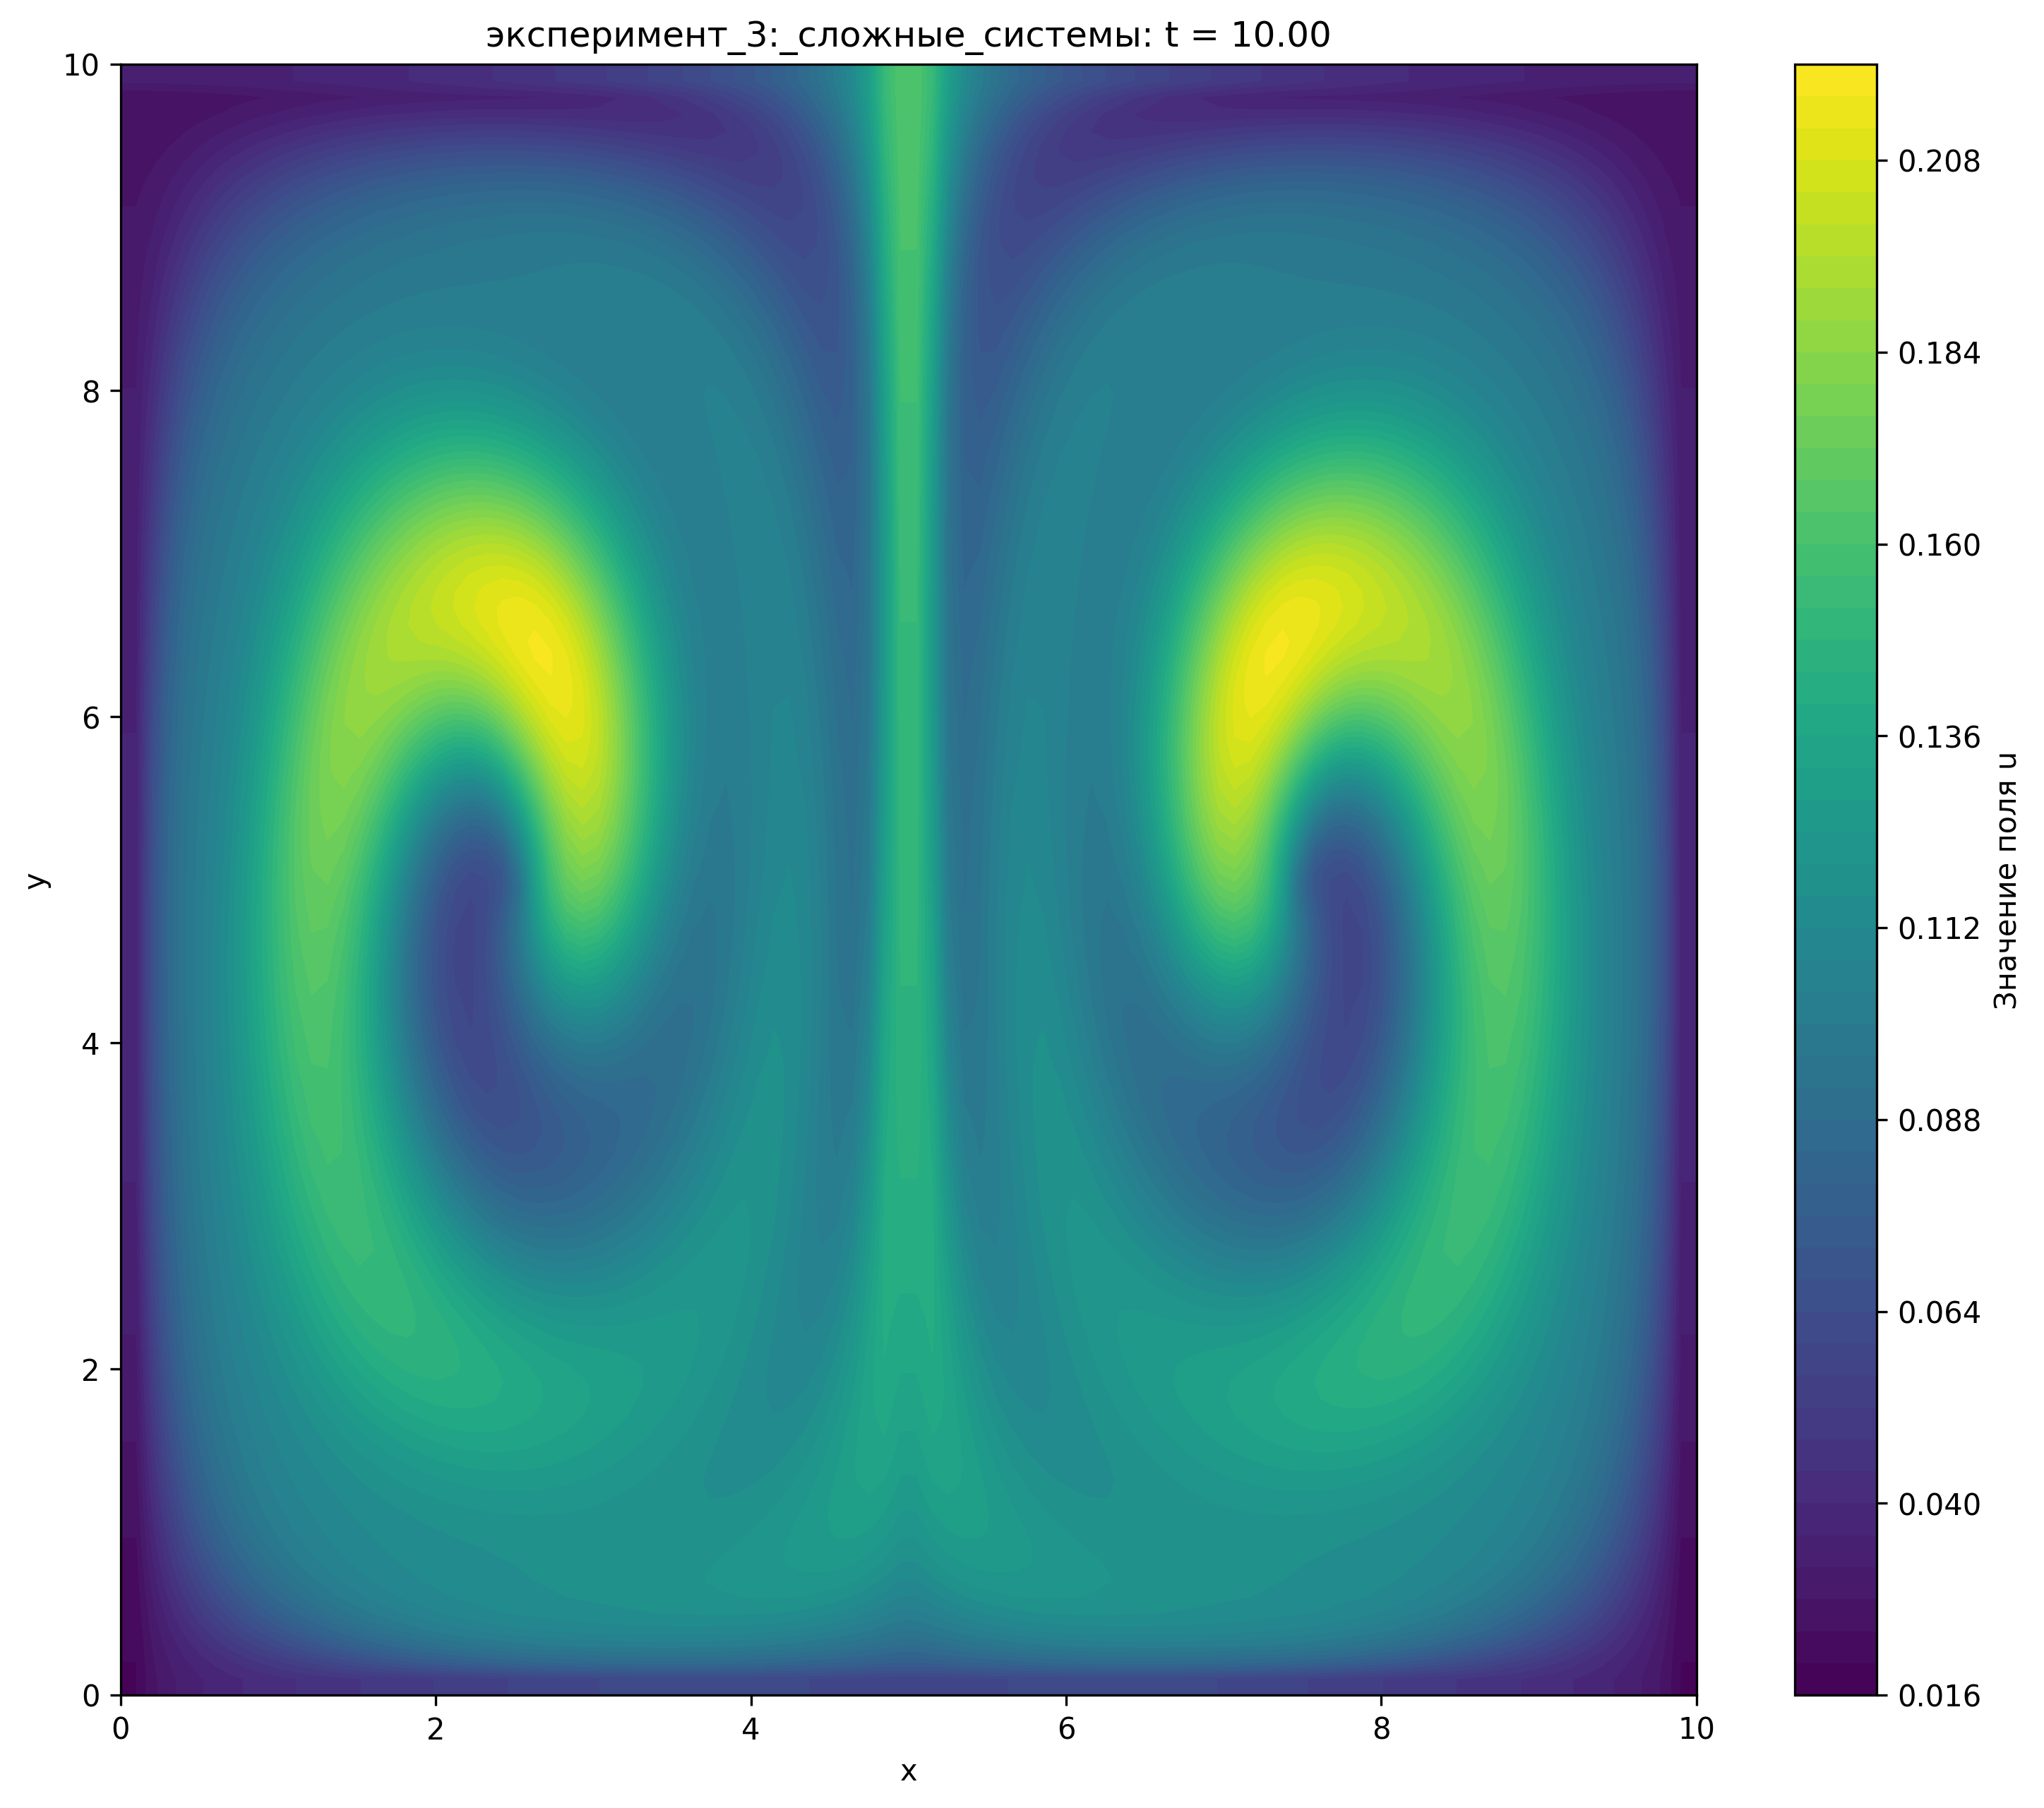
\includegraphics[width=0.7\textwidth]{imgs/эксперимент_3:_сложные_системы_t10.00.png}
	\caption{Скалярное поле \(u(x,y,T)\) в финальный момент времени (10) (вихревое течение)}
	\label{fig:div_final}
\end{figure}

\newpage

\section{Метод Лагранжевых точек}
\subsection{Описание численного метода}

В отличие от метода конечных разностей, лагранжев подход отслеживает движение частиц, несущих скалярную величину \( u \), по траекториям, определяемым полем скоростей. Основная идея заключается в решении задачи Коши для системы ОДУ:

\[
\frac{d \mathbf{x}}{dt} = \mathbf{v}(\mathbf{x}, t), \quad \mathbf{x}(0) = \mathbf{x}_0,
\]
где \( \mathbf{x}(t) = (x(t), y(t)) \) — положение частицы во времени, а \( \mathbf{v} = (v_x, v_y) \) — заданное поле скоростей.

Частицы не взаимодействуют и перемещаются независимо друг от друга. Величина \( u \) сохраняется вдоль траектории:

\[
\frac{du}{dt} = 0 \Rightarrow u(\mathbf{x}(t), t) = u(\mathbf{x}_0, 0).
\]

Для численного интегрирования используется метод Рунге–Кутты 4-го порядка (RK4):

\begin{equation}
	\begin{aligned}
		\mathbf{k}_1 &= \mathbf{v}(\mathbf{x}_n), \\
		\mathbf{k}_2 &= \mathbf{v}(\mathbf{x}_n + \tfrac{1}{2} \Delta t \mathbf{k}_1), \\
		\mathbf{k}_3 &= \mathbf{v}(\mathbf{x}_n + \tfrac{1}{2} \Delta t \mathbf{k}_2), \\
		\mathbf{k}_4 &= \mathbf{v}(\mathbf{x}_n + \Delta t \mathbf{k}_3), \\
		\mathbf{x}_{n+1} &= \mathbf{x}_n + \frac{\Delta t}{6} (\mathbf{k}_1 + 2\mathbf{k}_2 + 2\mathbf{k}_3 + \mathbf{k}_4).
	\end{aligned}
	\label{eq:rk4}
\end{equation}

\subsection{Реализация на Python}

Программа реализована на языке Python с использованием библиотек \texttt{numpy}, \texttt{matplotlib}, \texttt{scipy}. Структура кода включает:
\begin{itemize}
	\item \texttt{ParticleSet} — класс, отвечающий за координаты и значения частиц;
	\item \texttt{VelocityField} — статические методы для различных полей скоростей;
	\item \texttt{Integrator} — численные методы интегрирования траекторий (Euler, RK4);
	\item визуализацию движения частиц и их распределений;
	\item построение плотности \( u(x, y, t) \) через гауссово размывание или биннинг в сетку.
\end{itemize}

\begin{lstlisting}[language=Python, caption={Основной шаг метода Рунге–Кутты 4-го порядка для перемещения частиц}, label={lst:rk4_loop}]
	def rk4_step(x, y, vx_func, vy_func, dt):
	k1x = vx_func(x, y)
	k1y = vy_func(x, y)
	
	k2x = vx_func(x + 0.5 * dt * k1x, y + 0.5 * dt * k1y)
	k2y = vy_func(x + 0.5 * dt * k1x, y + 0.5 * dt * k1y)
	
	k3x = vx_func(x + 0.5 * dt * k2x, y + 0.5 * dt * k2y)
	k3y = vy_func(x + 0.5 * dt * k2x, y + 0.5 * dt * k2y)
	
	k4x = vx_func(x + dt * k3x, y + dt * k3y)
	k4y = vy_func(x + dt * k3x, y + dt * k3y)
	
	x_next = x + dt / 6 * (k1x + 2 * k2x + 2 * k3x + k4x)
	y_next = y + dt / 6 * (k1y + 2 * k2y + 2 * k3y + k4y)
	
	return x_next, y_next
\end{lstlisting}

\subsection{Описание экспериментов}

В экспериментах используются те же три стационарных поля скоростей (\ref{eq:vortex}), (\ref{eq:shear}), (\ref{eq:div}). Начальные положения частиц задаются равномерно либо случайно в пределах области \(\Omega = [0, 10]^2\). Начальные значения \( u \) задаются по формуле:

\[
u(\mathbf{x}_0) =
\begin{cases}
	1, & \text{если } \| \mathbf{x}_0 - \mathbf{x}_c \| \leq r, \\
	0, & \text{иначе},
\end{cases}
\]
где \(\mathbf{x}_c\) — центр круга, \(r\) — радиус.

\subsection{Визуализация результатов}

Для каждого эксперимента строятся:
\begin{itemize}
	\item карта начального положения и значений частиц;
	\item стримплот поля скоростей;
	\item финальное распределение частиц с учётом перемещения;
	\item по желанию: реконструированная плотность скалярной величины на сетке.
\end{itemize}

\subsection{Вихревое течение (Lagrangian)}
Поле используем то же, что и в эксперименте с разделёнными разностями ( рис. \ref{fig:vortex_velocity},  задаётся уравнением вихря (\ref{eq:vortex}).

В качестве начального распределения, используется круг с центром в точке (2.5 , 5) и радиусом 3 (\ref{fig:lg_vortex_begin}).
\begin{figure}
	\centering
	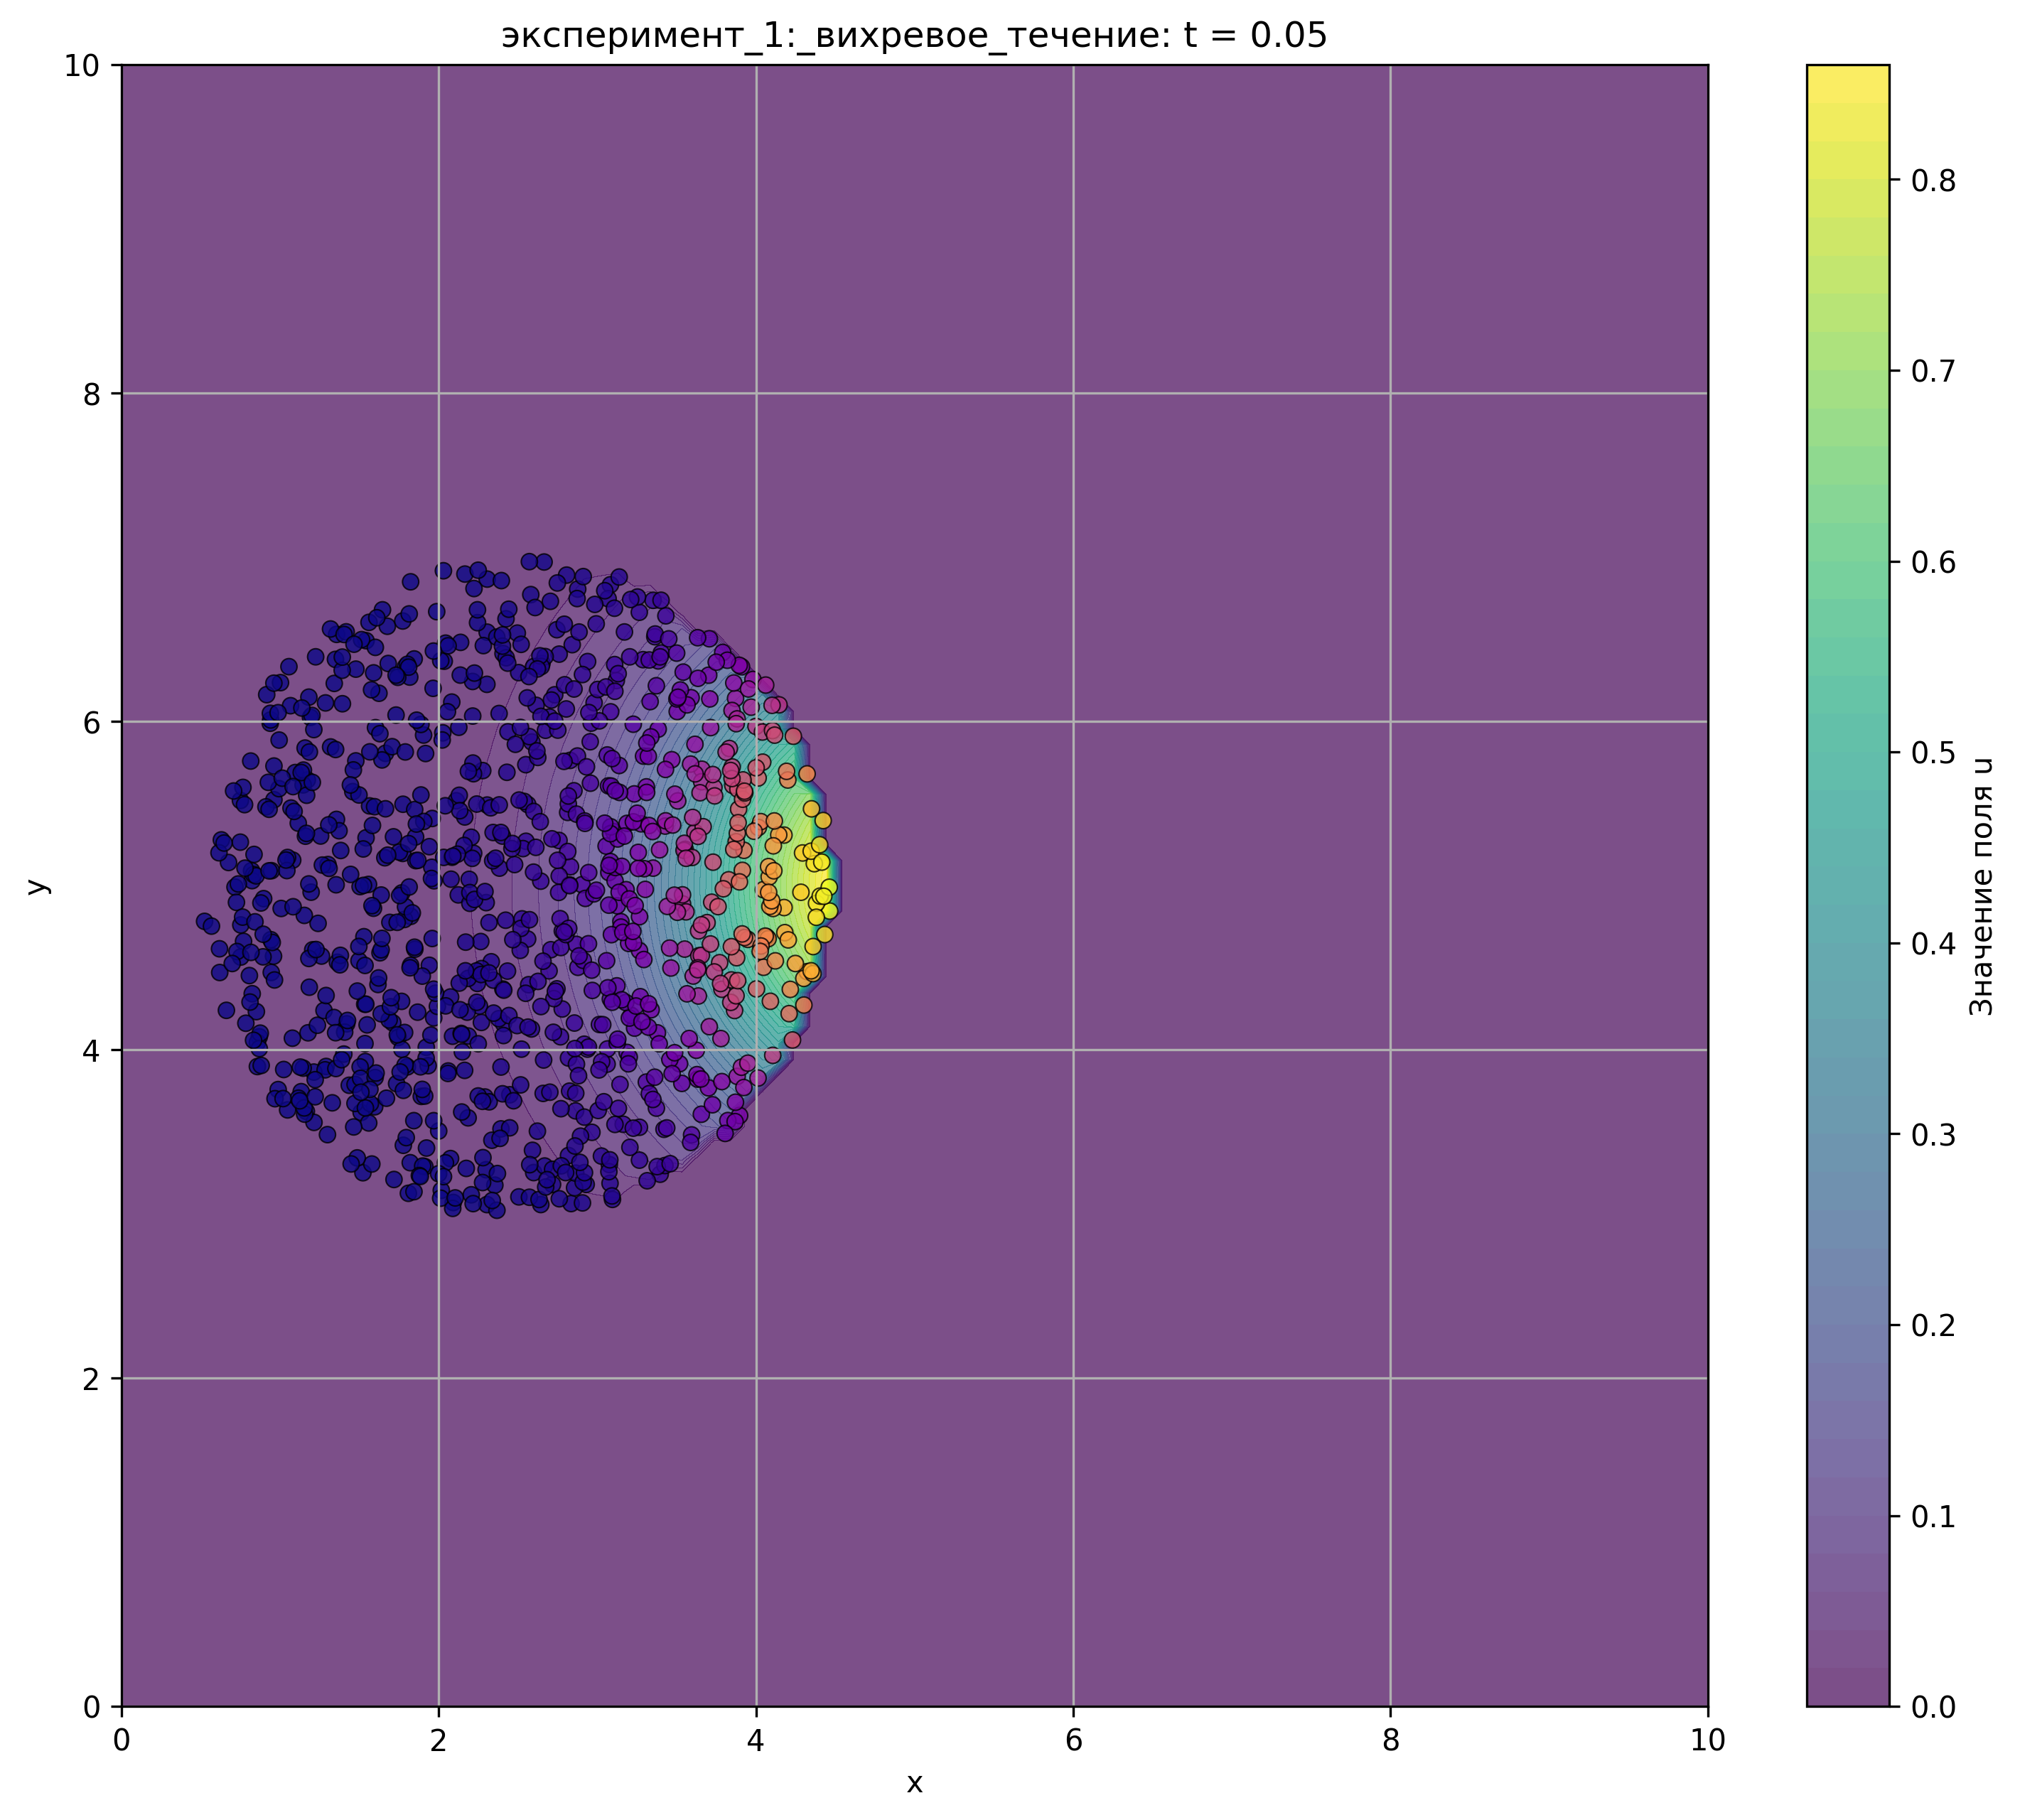
\includegraphics[width=0.7\textwidth]{imgs/lg/эксперимент_1:_вихревое_течение_t0.05.png}
	\caption{Начальное распределение частиц (вихревое течение)}
	\label{fig:lg_vortex_begin}
\end{figure}

Изображения промежуточных ходов представлены в приложении (ВСТАВИТЬ ССЫЛКУ НА ПРИЛОЖЕНИЕ).
Финального распределение представлено на рис. \ref{fig:lg_vortex_finall}.
\begin{figure}
	\centering
	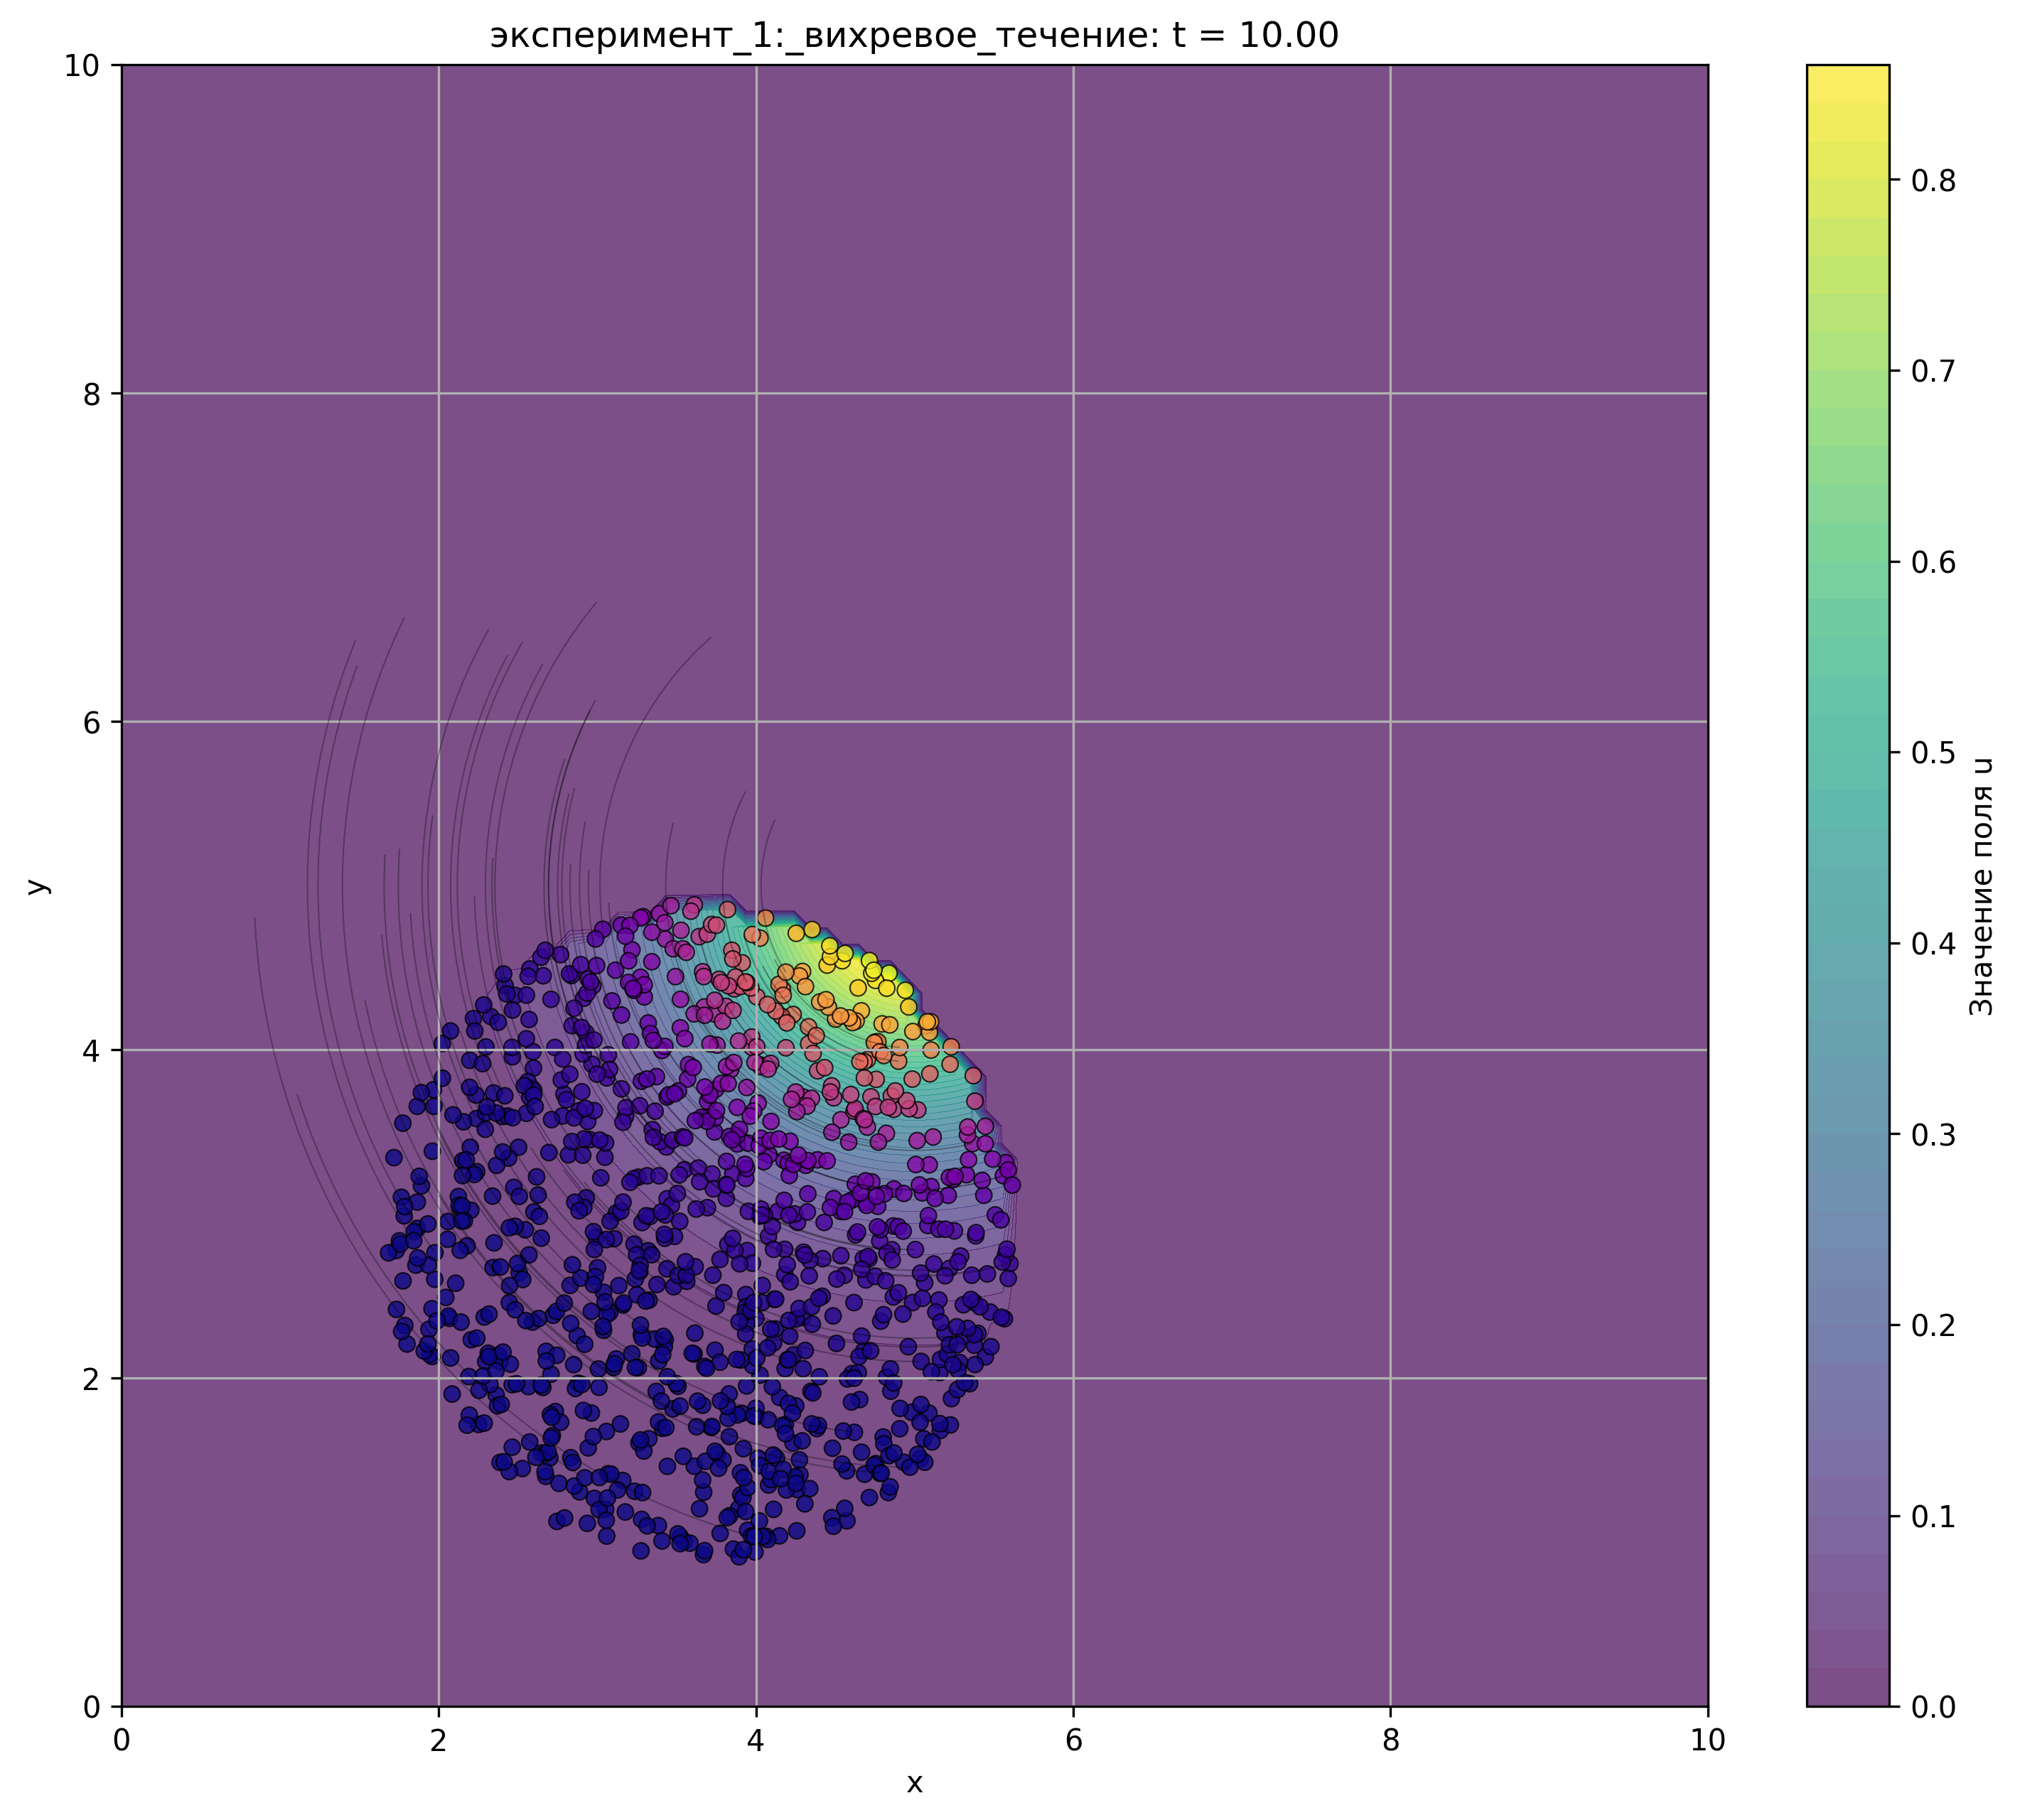
\includegraphics[width=0.7\textwidth]{imgs/lg/эксперимент_1:_вихревое_течение_t10.00.png}
	\caption{Финальное распределение частиц (вихревое течение)}
	\label{fig:lg_vortex_finall}
\end{figure}
Траектории 50 из 1000 точек представлены на рис. \ref{fig:lg_vortex_tr}
\begin{figure}
	\centering
	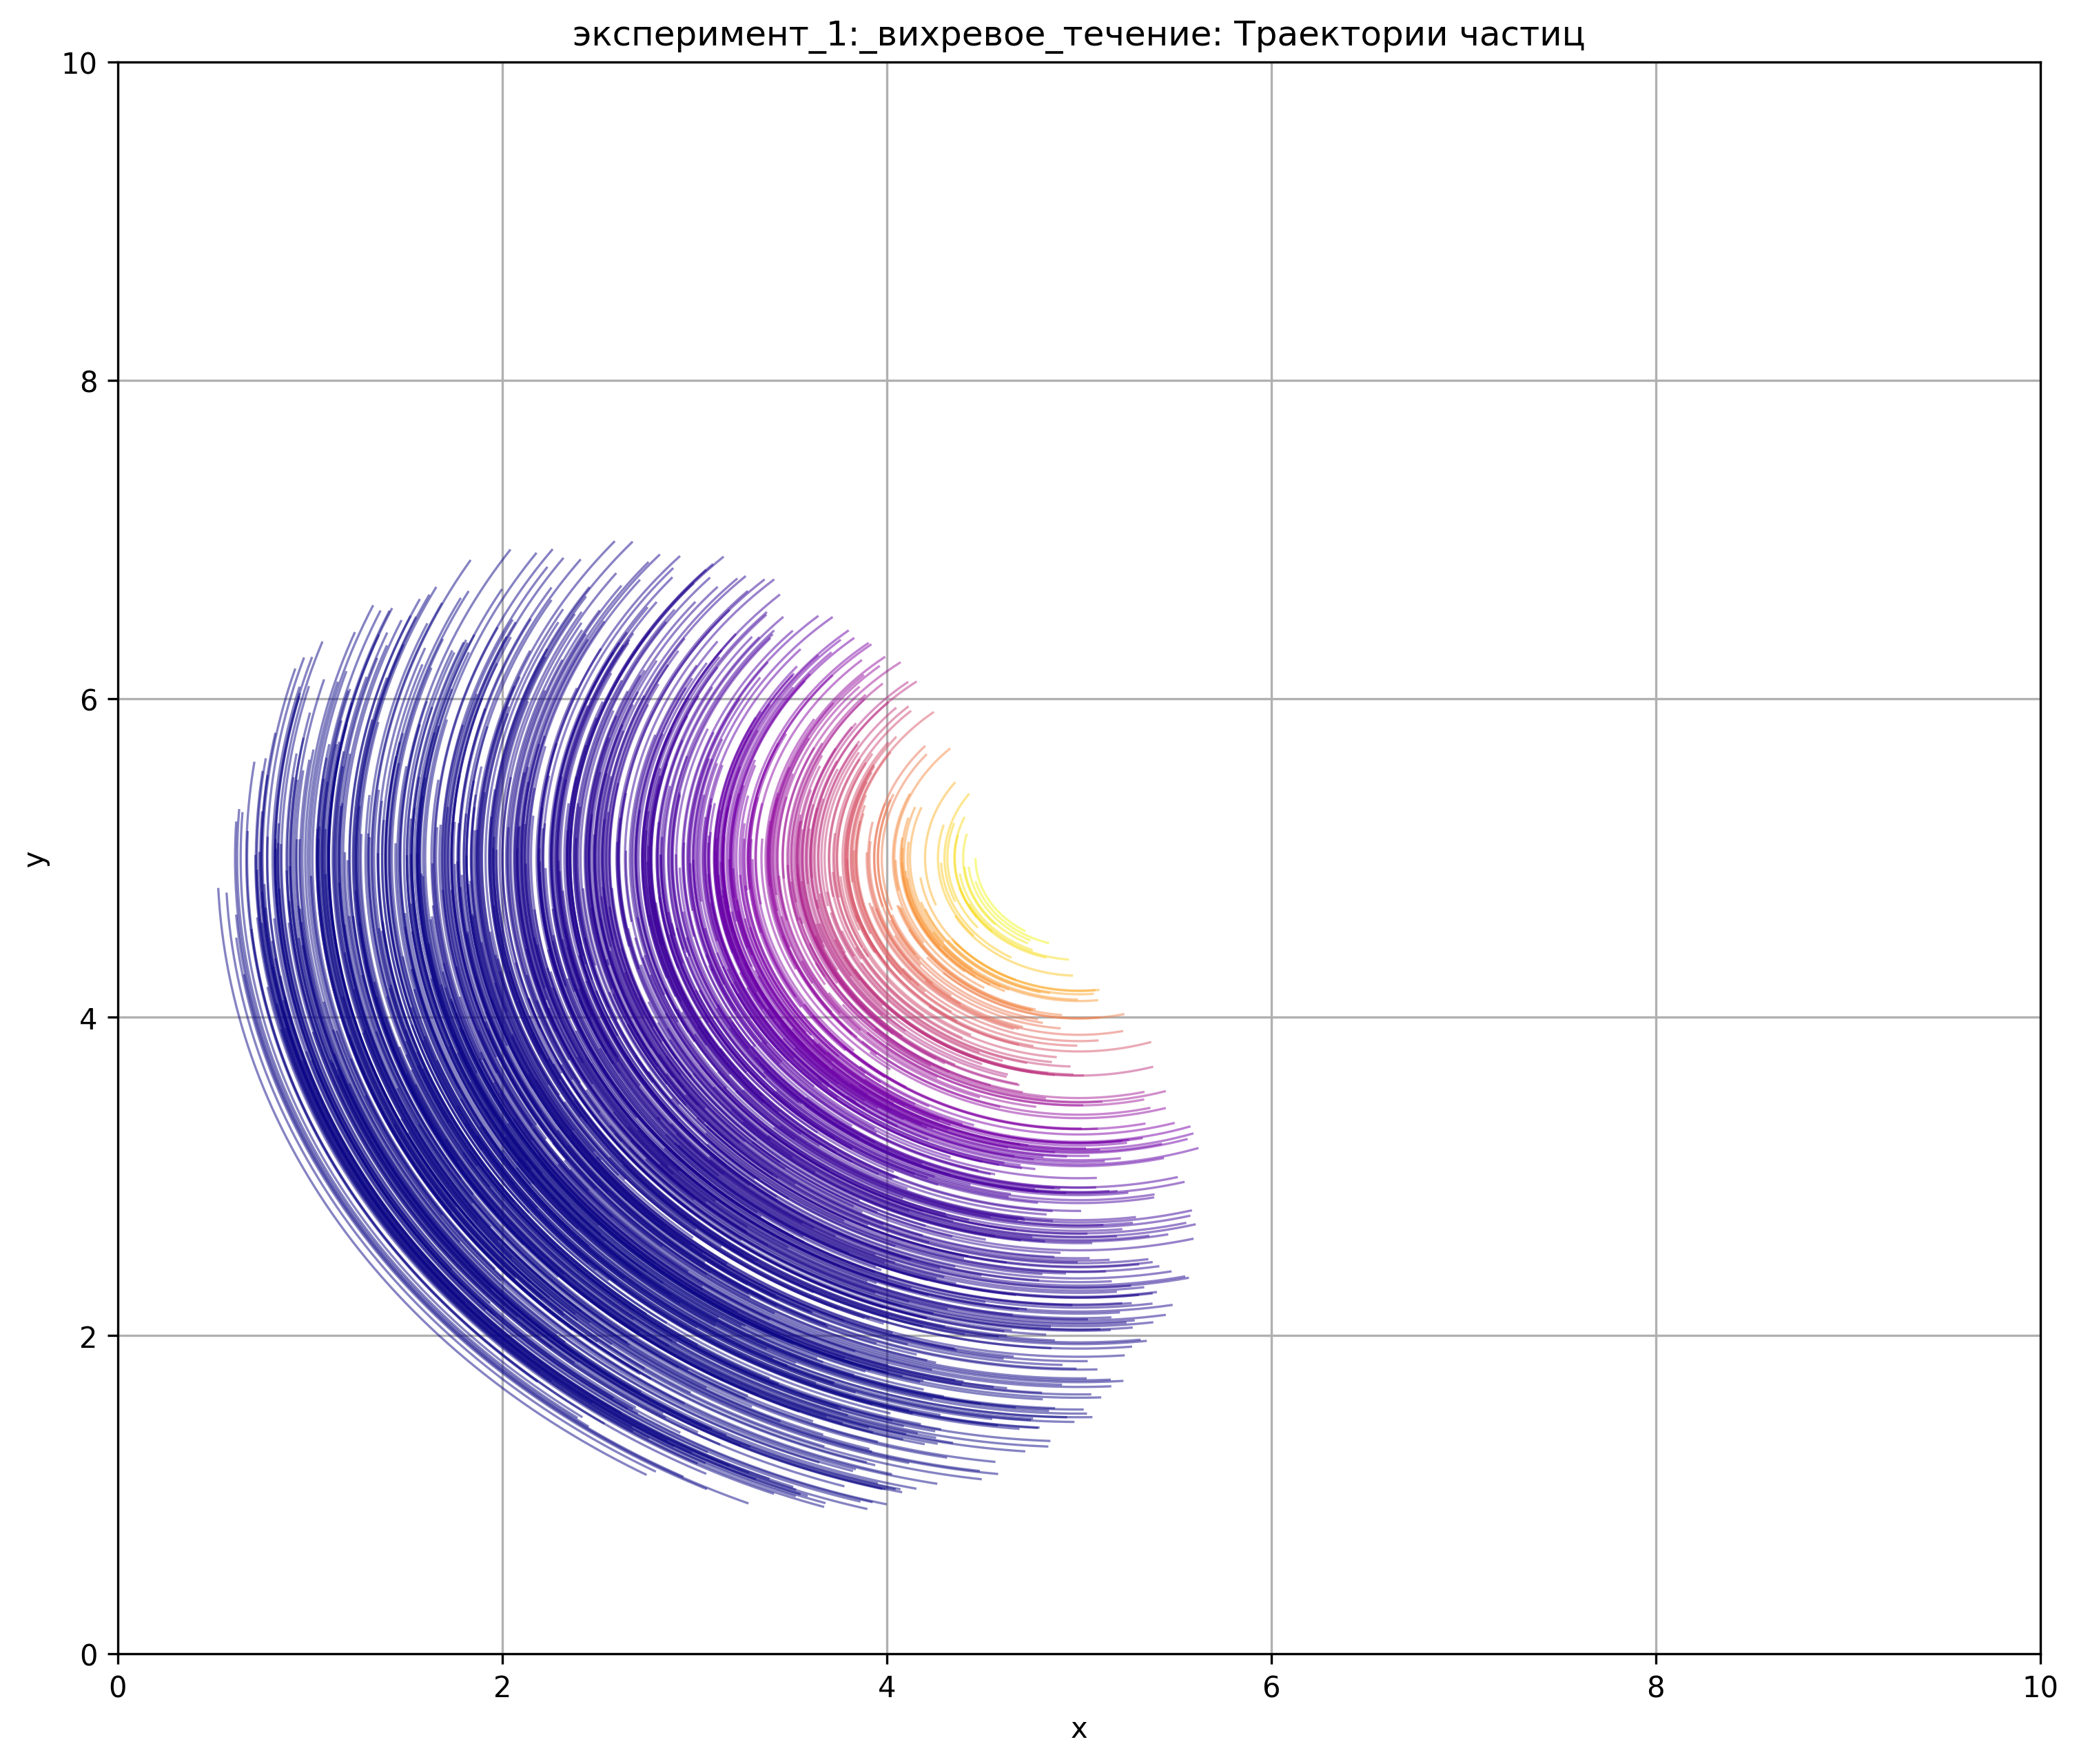
\includegraphics[width=0.7\textwidth]{imgs/lg/эксперимент_1:_вихревое_течение_trajectories.png}
	\caption{Финальное распределение частиц (вихревое течение)}
	\label{fig:lg_vortex_tr}
\end{figure}

\newpage
\subsection{Сдвиговое течение (Lagrangian)}

Поле используем то же, что и в эксперименте с разделёнными разностями (рис. \ref{fig:shear_velocity},  задаётся уравнением вихря (\ref{eq:shear}).

В качестве начального распределения, используется круг с центром в точке (5 , 5) и радиусом 2 (\ref{fig:lg_shaer_begin}). Дополнительно добавлена область вокруг распределения в виде квадрата для отрисовки поведения среды.
\begin{figure}
	\centering
	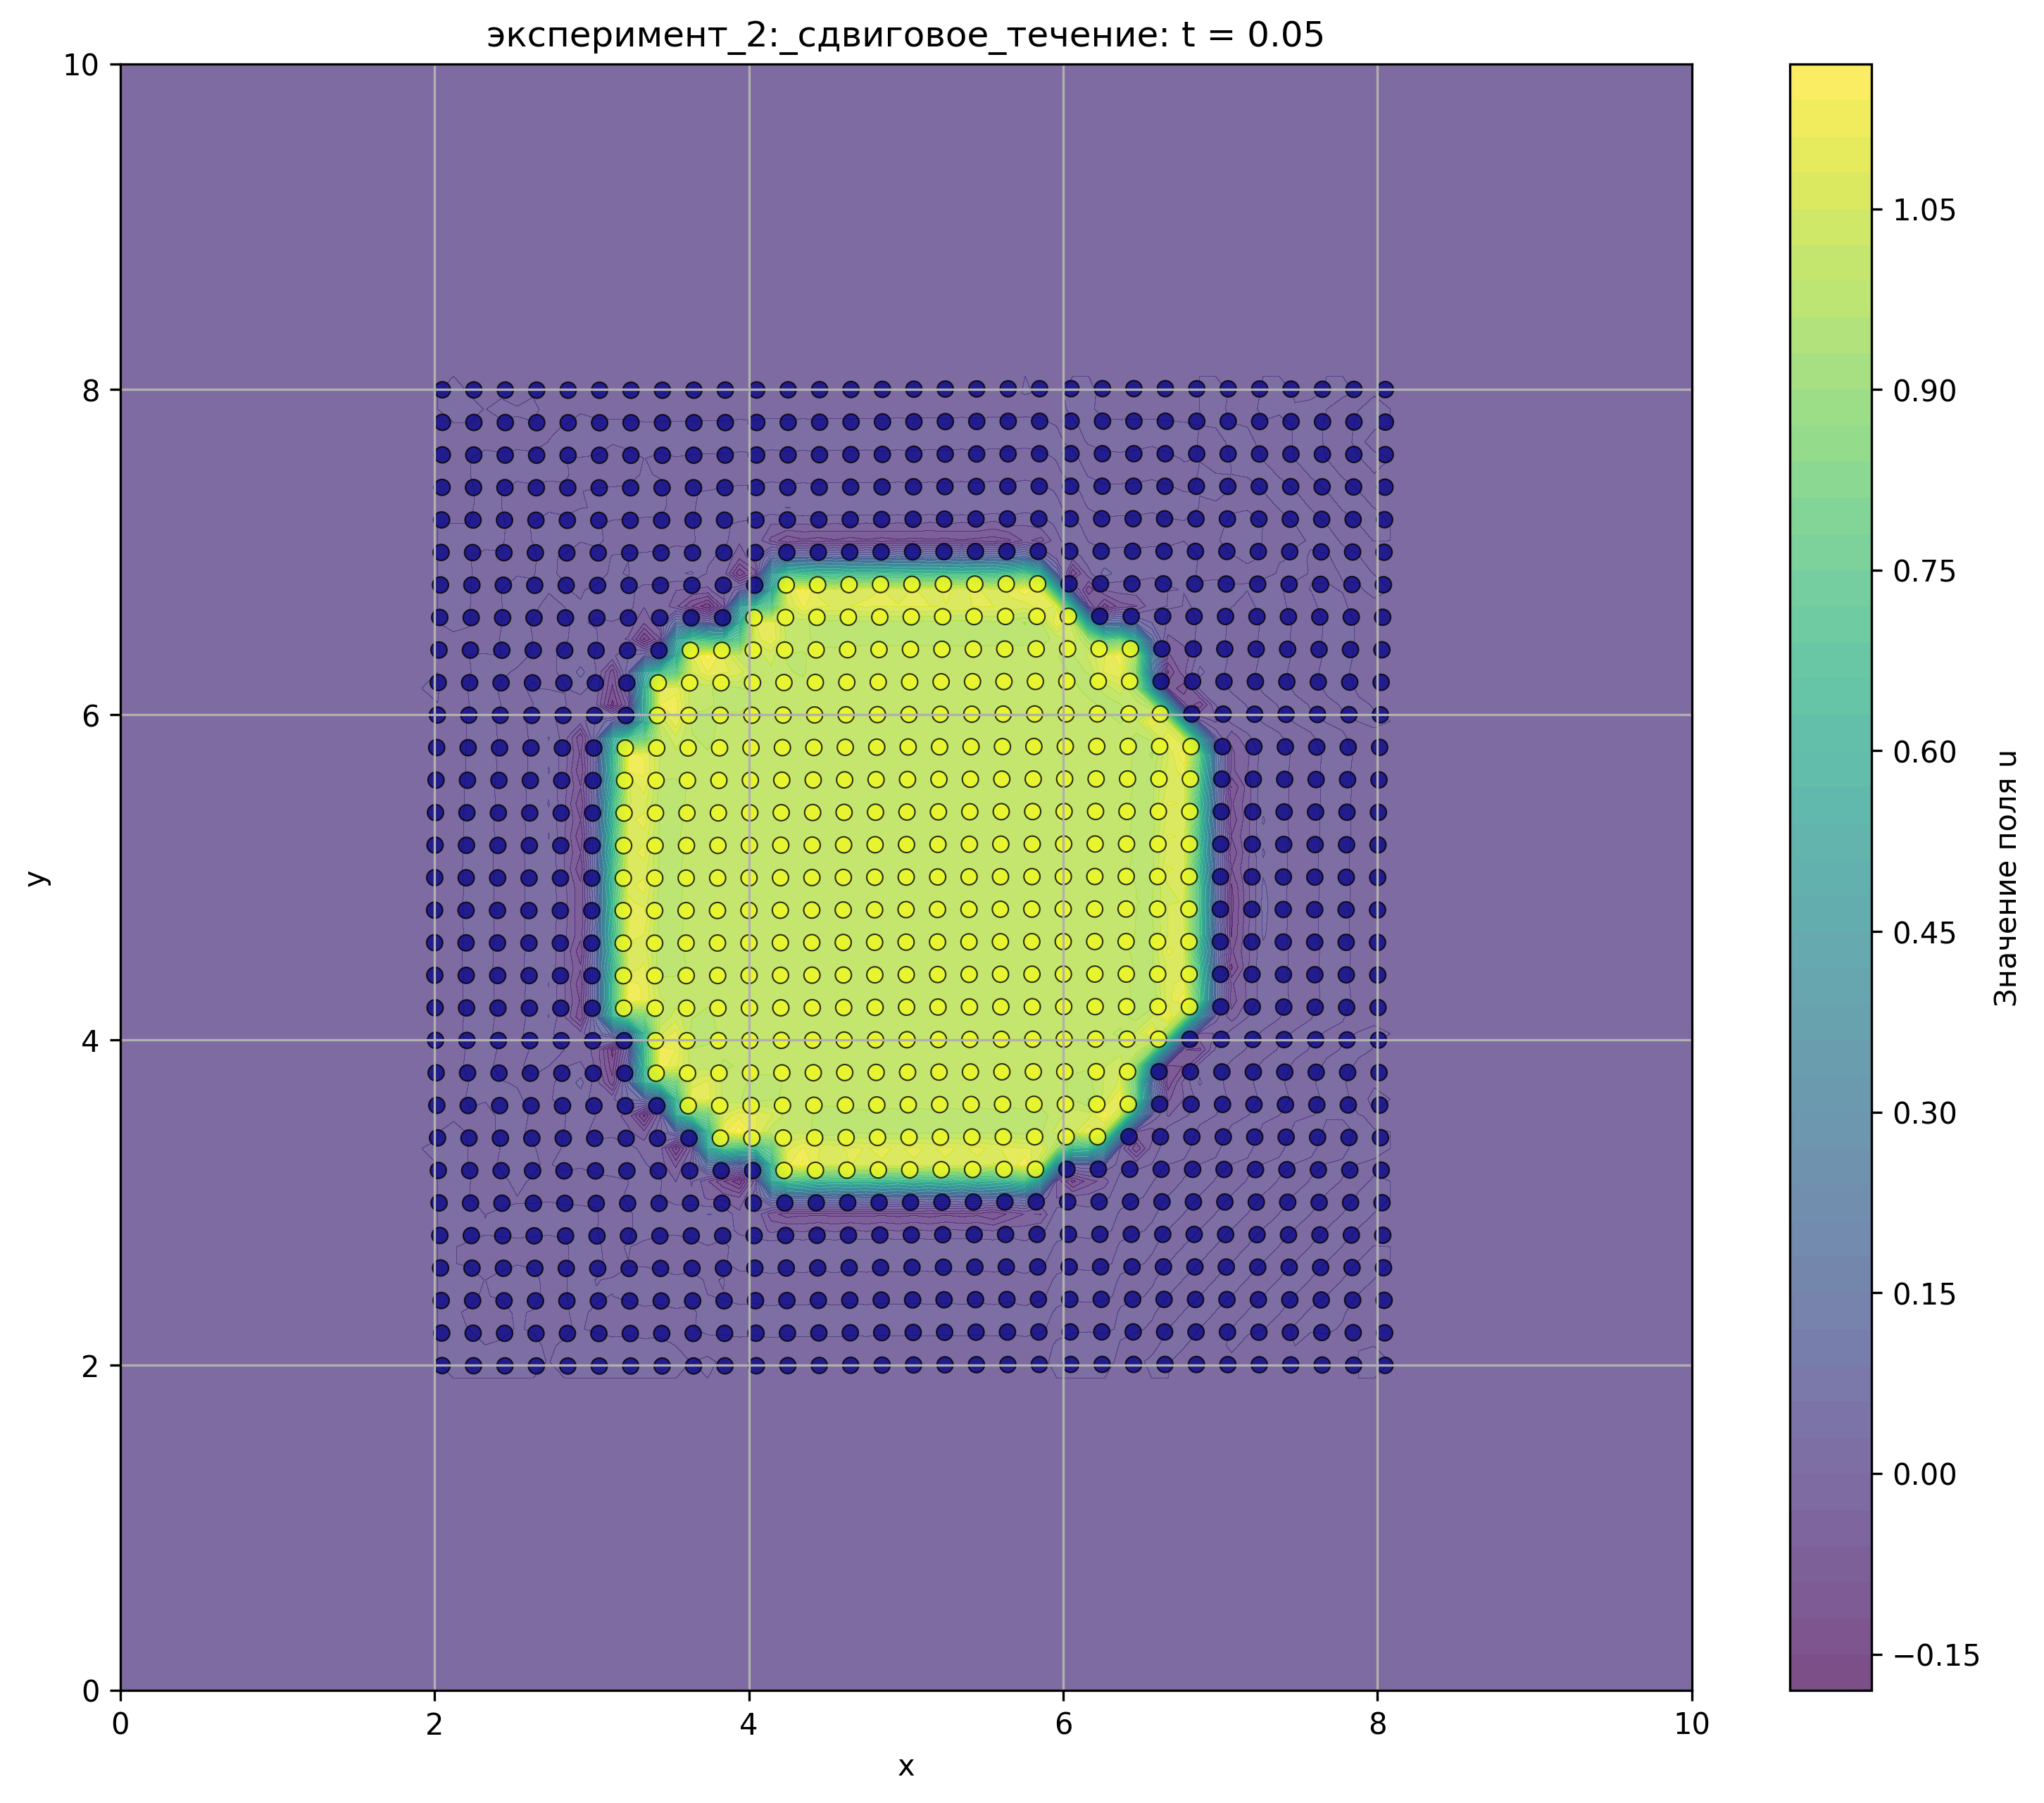
\includegraphics[width=0.7\textwidth]{imgs/lg/эксперимент_2:_сдвиговое_течение_t0.05.png}
	\caption{Начальное распределение частиц (сдвиговое течение)}
	\label{fig:lg_shaer_begin}
\end{figure}

Изображения промежуточных ходов представлены в приложении (ВСТАВИТЬ ССЫЛКУ НА ПРИЛОЖЕНИЕ).
Финального распределение представлено на рис. \ref{fig:lg_shaer_finall}.
\begin{figure}
	\centering
	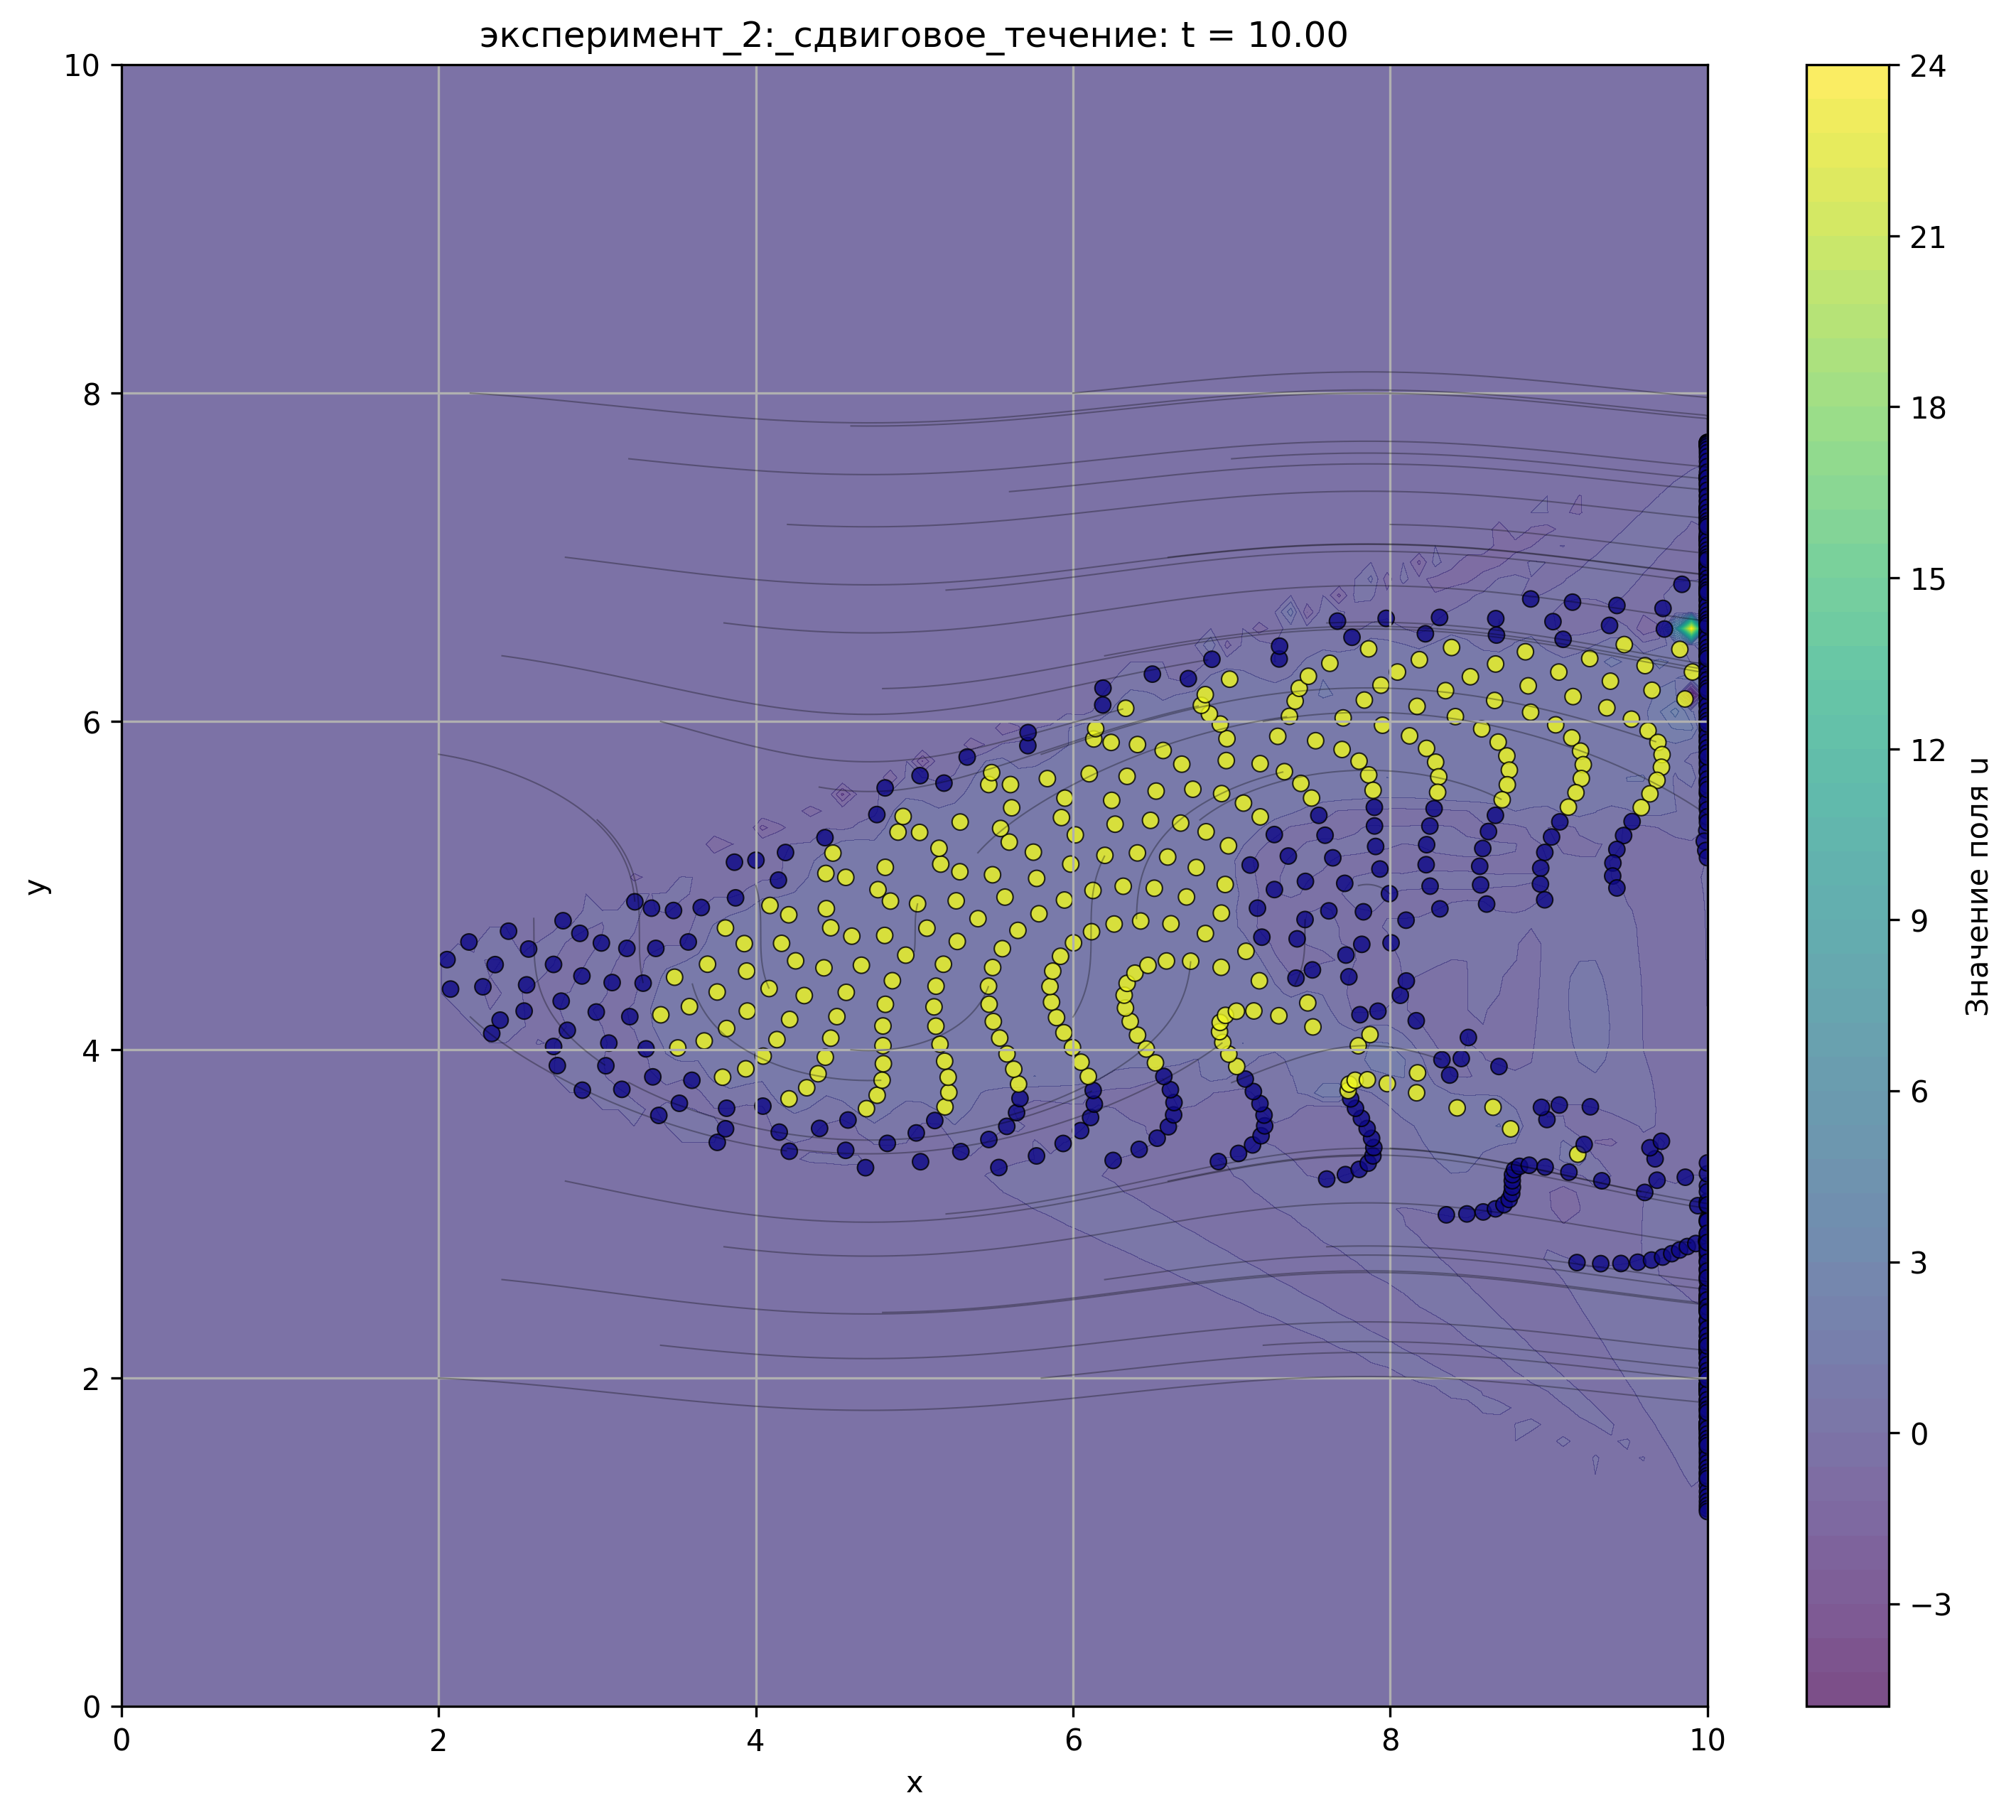
\includegraphics[width=0.7\textwidth]{imgs/lg/эксперимент_2:_сдвиговое_течение_t10.00.png}
	\caption{Финальное распределение частиц (сдвиговое течение)}
	\label{fig:lg_shaer_finall}
\end{figure}
Траектории 50 из 1000 точек представлены на рис. \ref{fig:lg_shaer_tr}
\begin{figure}
	\centering
	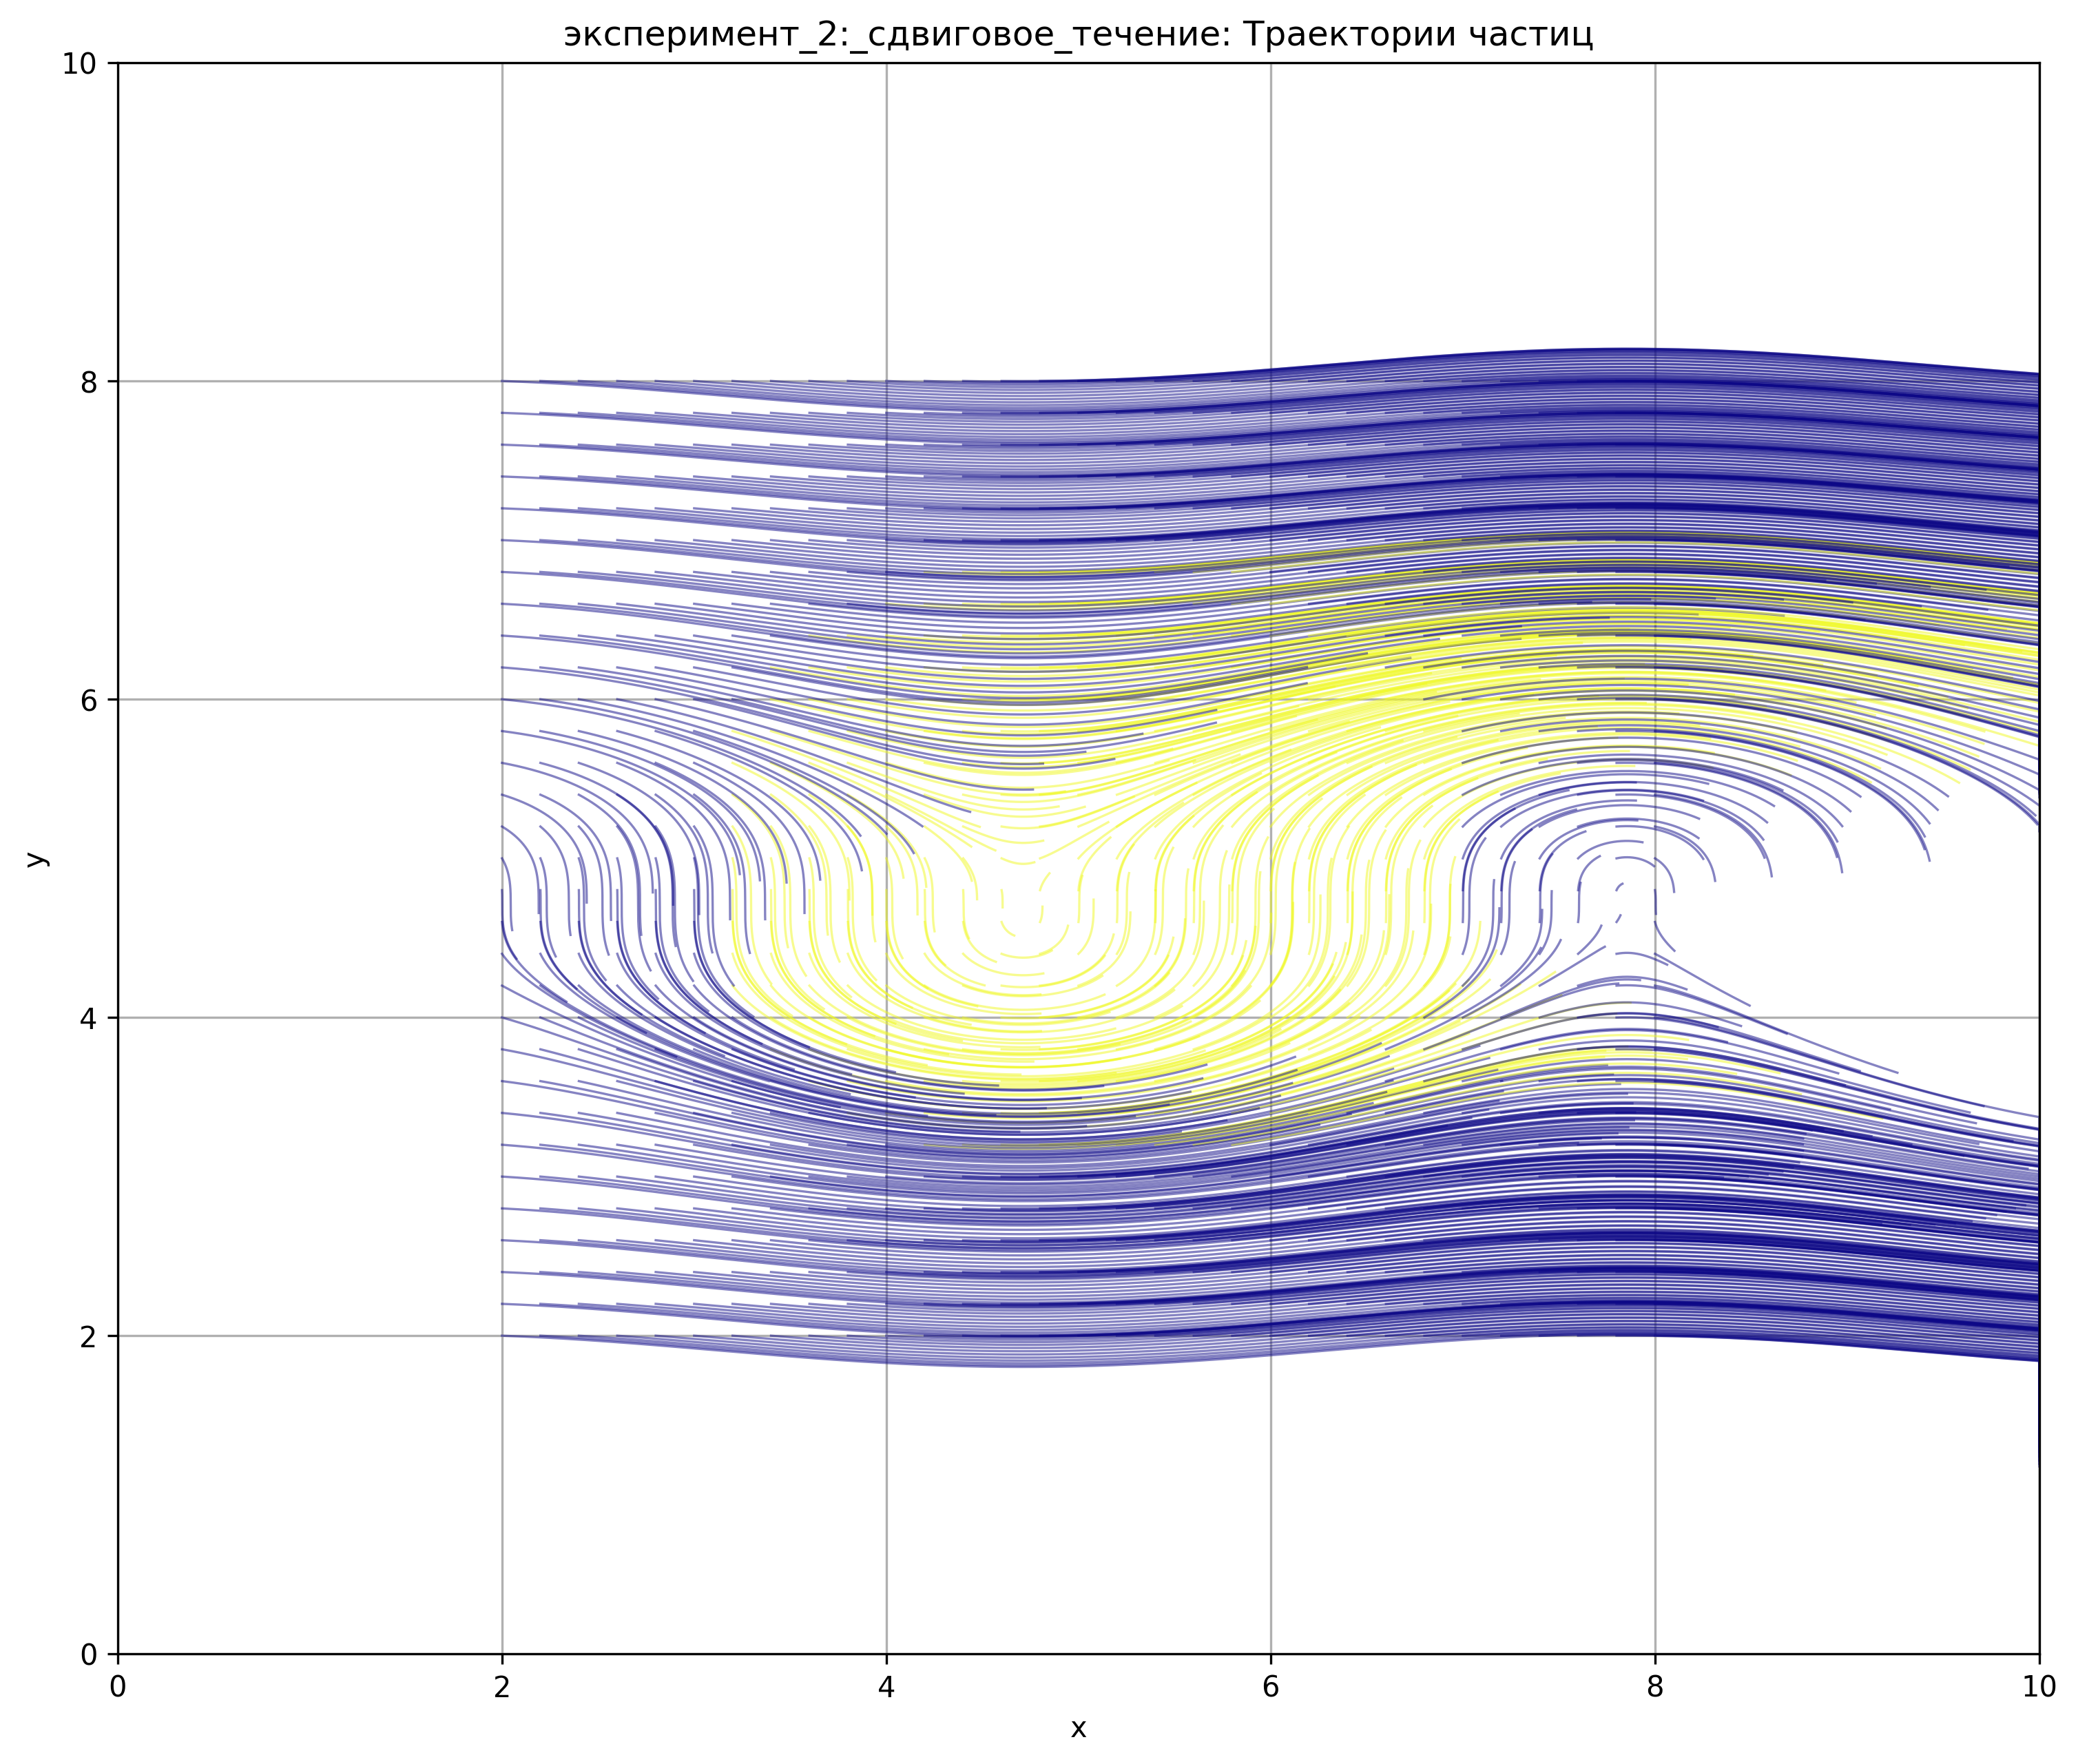
\includegraphics[width=0.7\textwidth]{imgs/lg/эксперимент_2:_сдвиговое_течение_trajectories.png}
	\caption{Траектории частиц (сдвиговое течение)}
	\label{fig:lg_shaer_tr}
\end{figure}

\newpage
\subsection{Дивергентное течение (Lagrangian)}
Поле используем то же, что и в эксперименте с разделёнными разностями (рис. \ref{fig:div_velocity},  задаётся уравнением вихря (\ref{eq:div}).

В качестве начального распределения, используется круг с центром в точке (5 , 5) и радиусом 2 (\ref{fig:lg_div_begin}). Дополнительно добавлена область вокруг распределения в виде квадрата для отрисовки поведения среды.
\begin{figure}
	\centering
	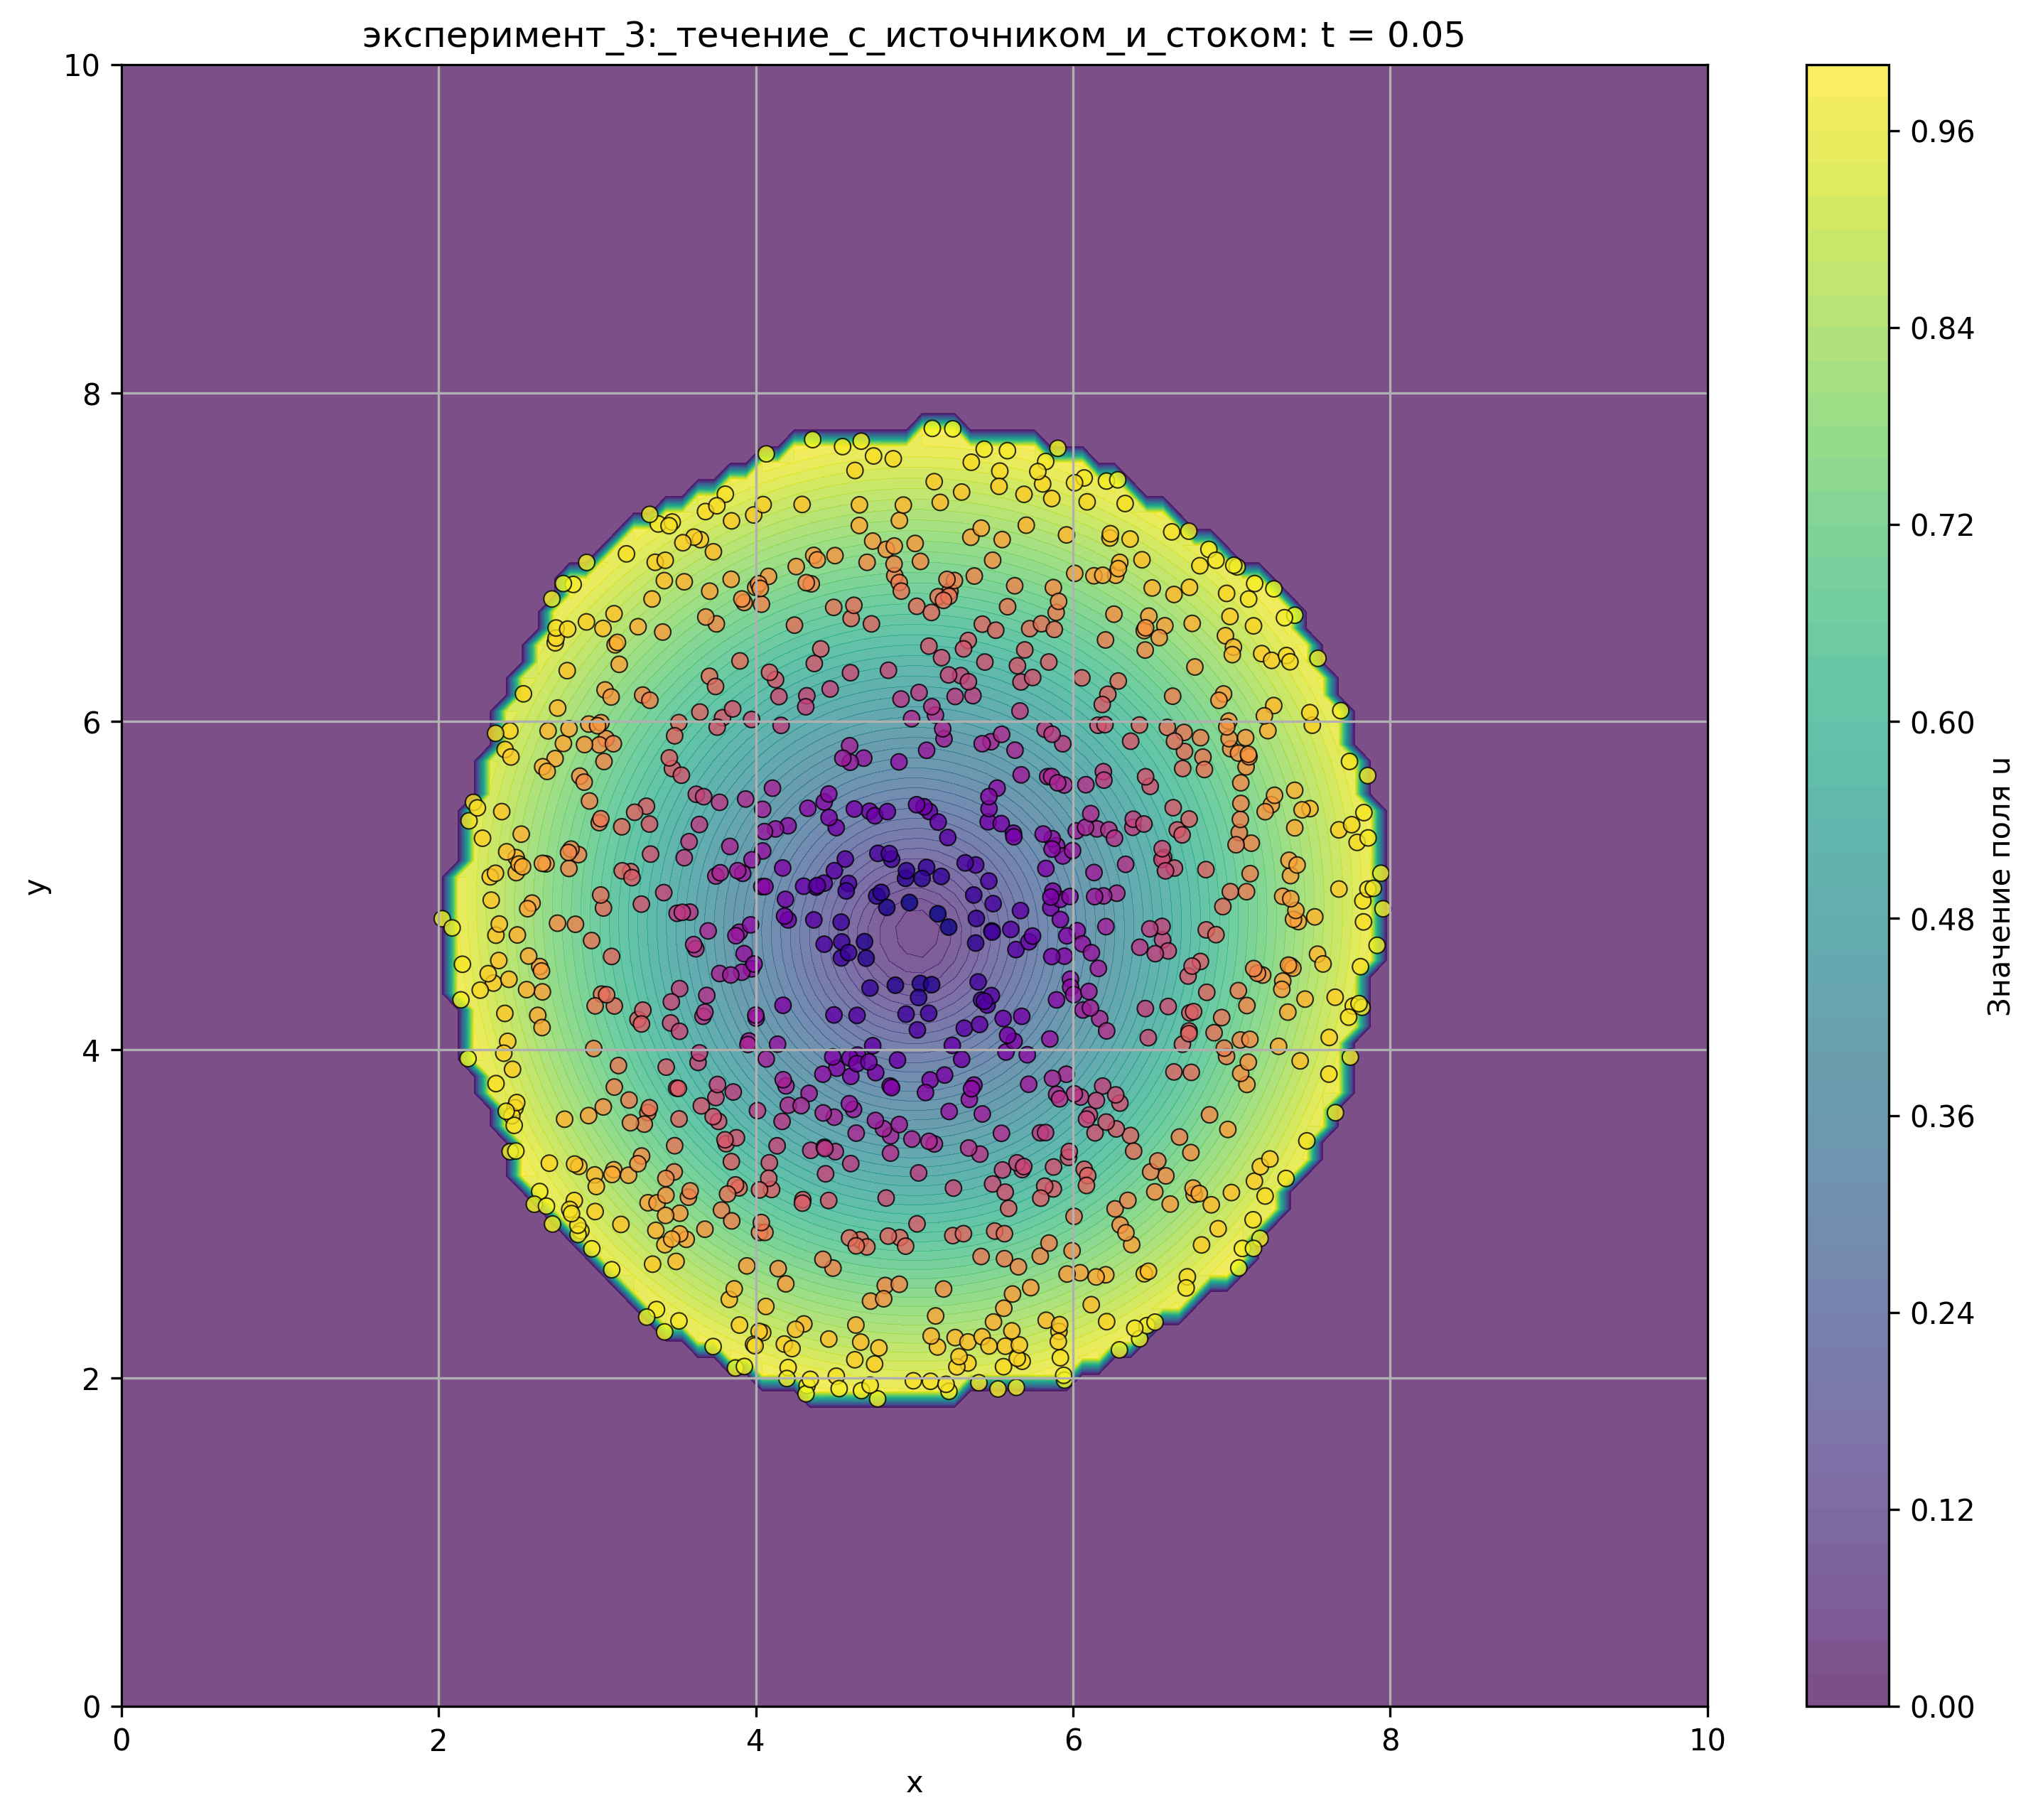
\includegraphics[width=0.7\textwidth]{imgs/lg/эксперимент_3:_течение_с_источником_и_стоком_t0.05.png}
	\caption{Начальное распределение частиц (дивергентное течение)}
	\label{fig:lg_div_begin}
\end{figure}

Изображения промежуточных ходов представлены в приложении (ВСТАВИТЬ ССЫЛКУ НА ПРИЛОЖЕНИЕ).
Финального распределение представлено на рис. \ref{fig:lg_div_finall}.
\begin{figure}
	\centering
	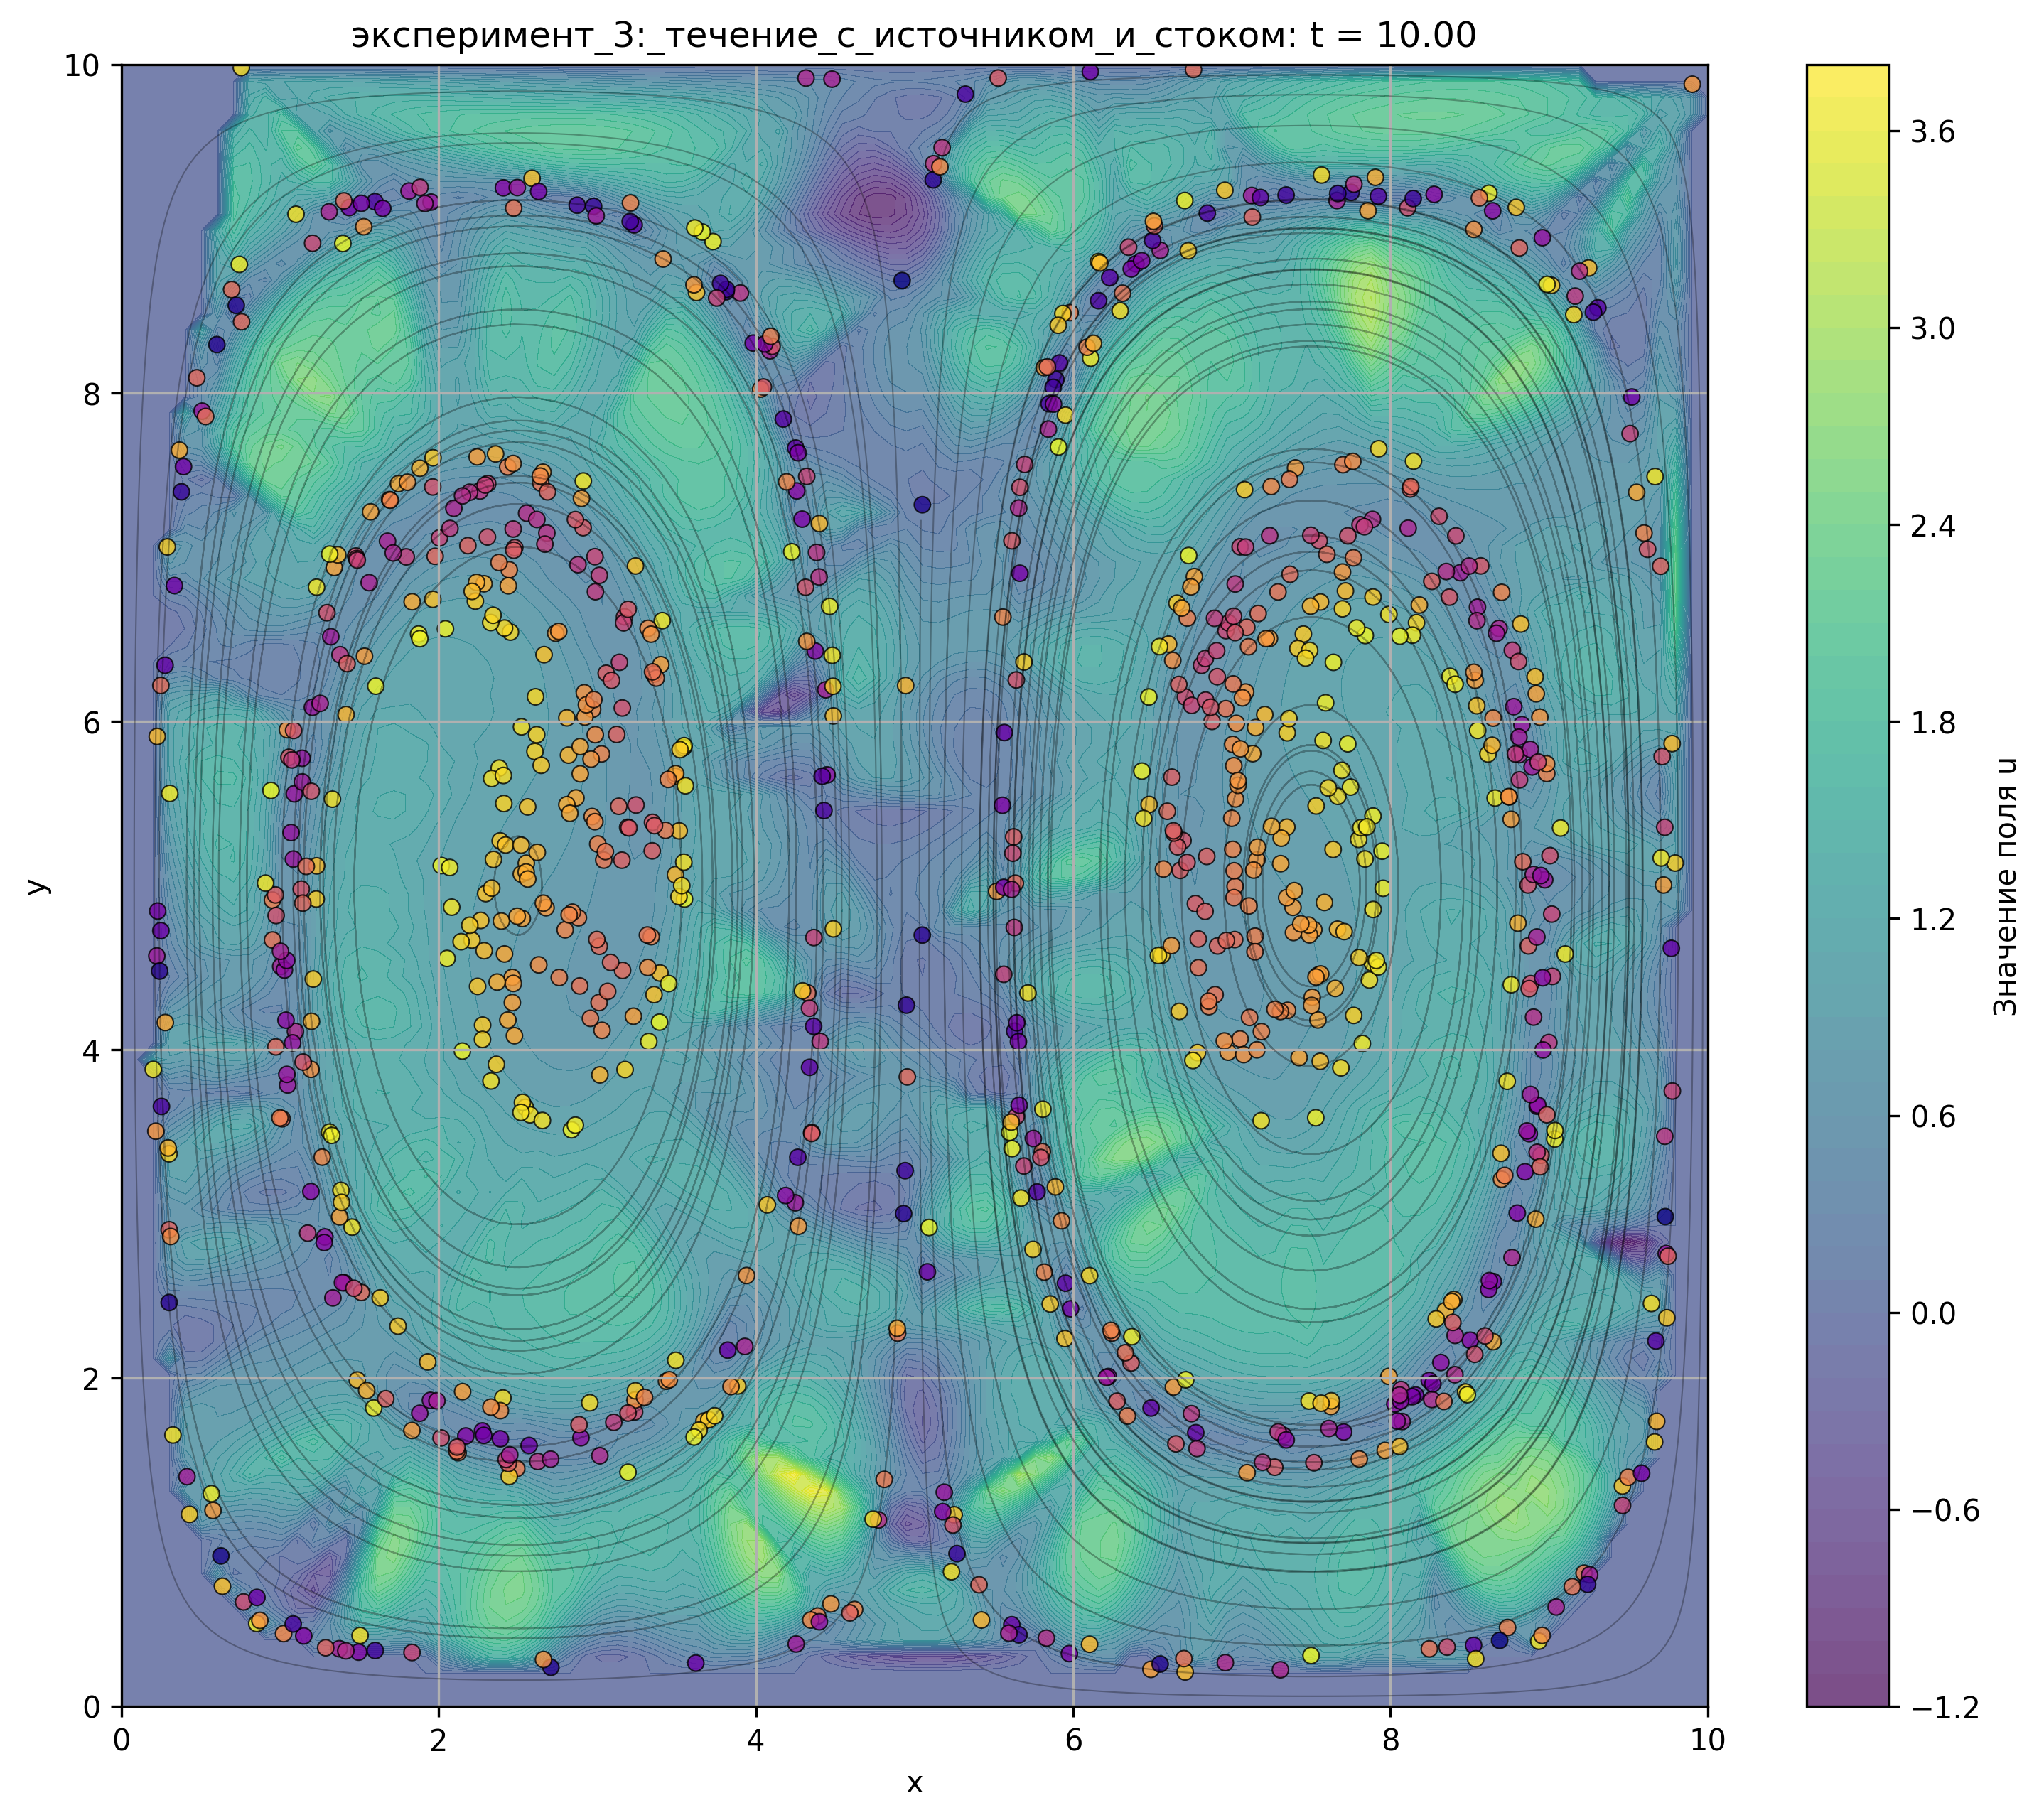
\includegraphics[width=0.7\textwidth]{imgs/lg/эксперимент_3:_течение_с_источником_и_стоком_t10.00.png}
	\caption{Финальное распределение частиц (дивергентное течение)}
	\label{fig:lg_div_finall}
\end{figure}
Траектории 50 из 1000 точек представлены на рис. \ref{fig:lg_div_tr}
\begin{figure}
	\centering
	\includegraphics[width=0.7\textwidth]{imgs/lg/эксперимент_3:_течение_с_источником_и_стоком_trajectories.png}
	\caption{Траектории частиц (дивергентное течение)}
	\label{fig:lg_div_tr}
\end{figure}

\newpage


\section{Выводы}

Метод конечных разностей позволяет качественно решать задачу переноса при условии соблюдения критерия CFL. Использование upwind-схем позволяет избежать осцилляций, но при этом может вызывать численное диффузионное размытие. Метод легко масштабируется и хорошо подходит для моделирования задач с заданным полем скоростей.

Метод лагранжевых точек (или лагранжевых частиц) обеспечивает высокую точность отслеживания переноса вещества или других скалярных величин в заданном поле скоростей. Вместо аппроксимации функции на фиксированной сетке, как в методе конечных разностей, метод отслеживает движение частиц по траекториям, определяемым полем скоростей. Это позволяет избежать численного диффузионного размытия и сохранять чёткие границы. Метод особенно эффективен при моделировании переноса в сильно неоднородных или турбулентных потоках.